\documentclass{bioinfo}
\usepackage{hhline}
\usepackage{fancyhdr}
\usepackage[normalem]{ulem}
\usepackage{tabularx}
\usepackage{graphicx}

\usepackage{pdfpages}
\usepackage[LY1]{fontenc}

\usepackage{soul}

\usepackage{atbegshi,picture}
\usepackage{lipsum}
\usepackage{mathtools}
\usepackage{amsmath}
\DeclarePairedDelimiter{\ceil}{\lceil}{\rceil}
\DeclarePairedDelimiter\floor{\lfloor}{\rfloor}

% Circles
\usepackage{tikz}
\newcommand*\circled[1]{\tikz[baseline=(char.base)]{
            \node[shape=circle,draw,inner sep=0pt,fill=black, text=white] (char) {#1};}}

% Commands for new text and comments
\newcommand\jgl[1]{\noindent{\color{blue} {\bf \fbox{JGL: }} {\it#1}}} % Juan
\newcommand\juan[1]{\noindent{\color{blue}#1}} % Juan

\newcommand\rev[1]{\noindent{{#1}}} % Modified after review
\usepackage{floatrow}
\floatplacement{figure}{H}
\floatsetup[table]{capposition=top}

%\AtBeginShipout{\AtBeginShipoutUpperLeft{  \put(\dimexpr\paperwidth-9.5cm\relax,-0.5cm){\makebox[0pt][r]{\color{blue}\framebox{version 7.2 --- 23 Nov 2020 --- 11:35}}}}}


\copyrightyear{2019} \pubyear{2019}

\access{Advance Access Publication Date: Day Month Year}
\appnotes{Manuscript Category}

\newcommand{\CA}[1]{\textbf{\color{magenta}{[#1]}}}
\newcommand{\alser}[1]{{\color{black}{#1}}}
\newcommand{\ts}[1]{{\color{cyan}TS: #1}}
\newcommand{\taha}[1]{{\color{cyan}#1}}
\newcommand{\taharm}[1]{{\color{cyan}\sout{#1}}\xspace}

\begin{document}
\firstpage{1}

\subtitle{Subject Section}

\title[SneakySnake: A Fast and Accurate Universal Genome Pre-Alignment Filter]{\alser{SneakySnake: A Fast and Accurate Universal Genome Pre-Alignment Filter for CPUs, GPUs, and FPGAs}}

\author[Alser \textit{et~al}.]{
Mohammed Alser\,$^{\text{\sfb 1}, \text{\sfb 2},\ast}$,
Taha Shahroodi\,$^{\text{\sfb 1}}$,
Juan G\'{o}mez-Luna\,$^{\text{\sfb 1}, \text{\sfb 2}}$,
\\Can Alkan\,$^{\text{\sfb 4},\ast}$, and \alser{Onur Mutlu\,$^{\text{\sfb 1}, \text{\sfb 2}, \text{\sfb 3}, \text{\sfb 4},\ast}$}

}
\address{
$^{\text{\sf 1}}$Department of Computer Science, ETH Zurich, Zurich 8006, Switzerland\\
$^{\text{\sf 2}}$Department of Information Technology and Electrical Engineering, ETH Zurich, Zurich 8006, Switzerland\\
$^{\text{\sf 3}}$Department of Electrical and Computer Engineering, Carnegie Mellon University, Pittsburgh 15213, PA, USA \\
$^{\text{\sf 4}}$Department of Computer Engineering, Bilkent University, Ankara 06800, Turkey \\
}

\corresp{$^\ast$To whom correspondence should be addressed.}

\history{Received on XXXXX; revised on XXXXX; accepted on XXXXX}

\editor{Associate Editor: XXXXXXX}

\corresp{$^\ast$To whom correspondence should be addressed.}

\history{Received on XXXXX; revised on XXXXX; accepted on XXXXX}

\editor{Associate Editor: XXXXXXX}

\abstract{\textbf{Motivation:} %Calculating the similarities between a pair of genomic sequences is one of the most fundamental computational steps in \alser{genomic analysis}.
%This step --called \emph{sequence alignment}-- is formulated as an \emph{approximate string matching} (ASM) problem, which is typically solved using computationally expensive dynamic programming algorithms. 
%In this work, 
We introduce \emph{SneakySnake}, a highly parallel and highly accurate pre-alignment filter that remarkably reduces the need for computationally costly sequence alignment. The key idea of SneakySnake is to reduce the \emph{approximate string matching} (ASM) problem to \alser{the} \emph{single net routing} (SNR) problem in VLSI chip layout. 
In \alser{the} SNR problem, we are interested in finding the optimal path that connects two terminals with the least routing cost on a special grid layout that contains obstacles. 
\alser{The} SneakySnake algorithm quickly solves the SNR problem and uses the found optimal path to decide whether {or not} performing sequence alignment is \alser{necessary}. Reducing the ASM problem into SNR also makes SneakySnake efficient to implement {on} 
%\emph{modern} high-performance computing architectures (
CPUs, GPUs, and FPGAs.\\
\textbf{Results:} SneakySnake significantly improves the accuracy of pre-alignment filtering by up to four orders of magnitude compared to the state-of-the-art pre-alignment filters, Shouji, GateKeeper, and SHD. 
{For} short sequences, SneakySnake accelerates Edlib (state-of-the-art implementation of Myers's bit-vector algorithm) and Parasail ({state-of-the-art} sequence aligner with {a} configurable scoring function), by up to 37.7$\times$ and 43.9$\times$ (>12$\times$ on average), respectively, {with} its CPU implementation, and by up to 413$\times$ and 689$\times$ (>400$\times$ on average), respectively, {with} {FPGA and GPU} acceleration.
{For} long sequences, {the CPU implementation of} SneakySnake accelerates Parasail and KSW2 (sequence aligner of minimap2) by up to 979$\times$ (276.9$\times$ on average) and 91.7$\times$ (31.7$\times$ on average), respectively.
%SneakySnake also accelerates the sequence alignment of minimap2, a state-of-the-art read mapper, {by up to 6.83$\times$ (4.67$\times$ on average) and 91.7$\times$ (31.7$\times$ on average) using short and long sequences, respectively,} and without requiring hardware acceleration. 
As SneakySnake does not replace sequence alignment, {users can still obtain \emph{all} capabilities (e.g., configurable scoring {functions}) of the aligner of their choice, unlike existing acceleration efforts that sacrifice some aligner capabilities}.\\
%for different \emph{scoring} functions, {surpassing existing acceleration efforts that greatly limit scoring function}.\\% that aim to accelerate sequence alignment.\\
%SneakySnake and Snake-on-Chip can be adopted for any bioinformatics pipeline that performs sequence alignment for verification. %SneakySnake and Snake-on-Chip reduce the execution time of state-of-the-art short read mapper, mrFAST \citep{alkan2009personalized}, by up to 2.93$\times$ and 7.57$\times$, respectively. \\
\textbf{Availability:} https://github.com/CMU-SAFARI/SneakySnake\\
\textbf{Contact:} \href{alserm@inf.ethz.ch}{alserm@inf.ethz.ch}, \href{calkan@cs.bilkent.edu.tr}{calkan@cs.bilkent.edu.tr}, \href{omutlu@ethz.ch}{omutlu@ethz.ch}\\
\textbf{Supplementary information:} Supplementary data is available at \emph{Bioinformatics} online.
\\}
\maketitle

\section{Introduction} \label{sec:introduction}
%The ability to quickly analyze the overwhelming amounts of sequencing data enables several scientific advancements in personalized medicine and understanding genomic contributions to health across population \citep{hindorff2018prioritizing}. 
One of the most fundamental computational steps in most genomic analyses is {\emph{sequence alignment}}~\citep{alser2020technology, senol2019nanopore}. 
This step is formulated as \alser{an} \emph{approximate string matching} (ASM) problem \citep{navarro2001guided} and \alser{it calculates: (1) \emph{edit distance} between two given sequences, (2) type of each edit (i.e., insertion, deletion, or substitution), and (3) location of each edit in one of the two given sequences.}
Edit distance is defined as the minimum number of edits needed to convert one sequence into the other \citep{levenshtein1966binary}. \alser{These edits result from both sequencing errors \citep{firtina2020apollo} and genetic variations \citep{10002015global}. }
Edits can have different weights, based on a user-defined \emph{scoring} function, to allow favoring one edit type over \alser{another} \citep{wang2011comparison}. 
Sequence alignment involves a \emph{backtracking step}, which calculates an ordered list of characters representing the location and type of each possible edit operation required to change one of the two given sequences into the other. 
As any two sequences can have several different arrangements of the edit operations, we need to examine all possible \emph{prefixes} of the two input sequences and keep track of the pairs of prefixes that provide a minimum edit distance. 
%Enumerating all possible prefixes is necessary for tolerating edits.
Therefore, sequence alignment approaches are typically implemented as dynamic programming (DP) algorithms to avoid re-examining the same prefixes {many times} \citep{alser2020technology,eddy2004dynamic}. 
DP-based \alser{sequence alignment algorithms}, such as Needleman-Wunsch \citep{needleman1970general}, are computationally expensive as they have quadratic time and space complexity (i.e., O($m^2$) for a sequence length of $m$). Many attempts were made to boost the performance of existing sequence aligners. Recent attempts tend to follow one of two \alser{key directions}{, as we comprehensively survey} in~\citep{alser2020accelerating}: (1) Accelerating the DP algorithms using hardware accelerators and (2) Developing pre-alignment filtering heuristics that reduce the need for the DP algorithms, given an edit distance threshold.

Hardware accelerators include building aligners that use 1) multi-core and SIMD (single instruction multiple data) capable central processing units (CPUs), such as Parasail \citep{daily2016parasail}.
The classical DP algorithms can also be accelerated by calculating a bit representation of the DP matrix and processing its bit-vectors in parallel, such as Myers's bit-vector algorithm \citep{myers1999fast}. To our knowledge, Edlib \citep{vsovsic2017edlib} is currently the best-performing implementation of Myers's bit-vector algorithm. 
Other hardware accelerators include 2) graphics processing units (GPUs), such as GSWABE \citep{liu2015gswabe}, 3) field-programmable gate arrays (FPGAs), such as FPGASW \citep{fei2018fpgasw}, or 4) {processing-in-memory architectures that enable performing computations inside the memory chip and alleviate the need for transferring the data to the CPU cores, such as} GenASM~\citep{senolcalimicro2020}. However, many of these efforts either simplify the scoring function as in Edlib, or only take into account accelerating the computation of the DP matrix without performing the backtracking step as in \citep{ chen2014accelerating}. Different and more sophisticated scoring functions are typically needed to better quantify the similarity between two sequences \citep{wang2011comparison}. The backtracking step involves unpredictable and irregular memory access patterns, which pose a difficult challenge for efficient hardware implementation.

Pre-alignment filtering heuristics aim to quickly eliminate some of the dissimilar sequences before using the computationally-expensive optimal alignment algorithms.
Existing pre-alignment filtering techniques are either: 1) slow and they suffer from a limited sequence length ($\leq128 bp$), such as SHD \citep{xin2015shifted}, or 2) inaccurate after some edit distance threshold, such as GateKeeper \citep{alser2017gatekeeper} and MAGNET \citep{alser2017magnet1}.
{Highly-parallel filtering can also be achieved using processing-in-memory architectures, as in} GRIM-Filter~\citep{kim2018grim}.
Shouji \citep{alser2019shouji} is currently the best-performing FPGA pre-alignment filter in terms of both accuracy and execution time.
%We provide full descriptions of these two key directions of accelerating sequence alignment in \textcolor{red}{Supplementary Material, Section 5}.

%\textbf{Hardware accelerators are becoming increasingly popular for speeding up the computationally expensive sequence aligners} \citep{aluru2014review, sandes2016parallel, al2017survey, ng2017reconfigurable}. 
%Hardware accelerators include multi-core and SIMD (single instruction multiple data) capable central processing units (CPUs), graphics processing units (GPUs), and field-programmable gate arrays (FPGAs). 
%The classical DP algorithms are typically accelerated by computing only the necessary regions (i.e., diagonal vectors) of the DP matrix rather than the entire matrix, as proposed in Ukkonen's banded algorithm \citep{ukkonen1985algorithms}. 
%The number of the diagonal bands required for computing the DP matrix is 2$E$+1, where $E$ is a user-defined edit distance threshold. The banded algorithm is still beneficial even with its recent sequential implementations as in Edlib \citep{vsovsic2017edlib}. 
%\alser{Edlib is implemented in C for standard CPUs and it calculates the banded Levenshtein distance}. 
%Parasail \citep{daily2016parasail} exploits both Ukkonen's banded algorithm and SIMD-capable CPUs to compute a banded alignment for a sequence pair with a user-defined scoring function. SIMD instructions offer significant parallelism to the matrix computation by executing the same vector operation on multiple operands at once. Multi-core architecture of CPUs and GPUs provides the ability to compute alignments of many sequence pairs independently and concurrently \citep{georganas2015meraligner, liu2015gswabe}. GSWABE \citep{liu2015gswabe} exploits GPUs (Tesla K40) for a highly-parallel computation of global alignment with a user-defined scoring function. CUDASW++ 3.0 \citep{liu2013cudasw++} exploits the SIMD capability of both CPUs and GPUs (GTX690) to accelerate the computation of the Smith-Waterman algorithm with a user-defined scoring function. CUDASW++ 3.0 provides only the optimal score, not the optimal alignment (i.e., no backtracking step). Other designs, for instance FPGASW \citep{fei2018fpgasw}, exploit the very large number of hardware execution units in FPGAs (Xilinx VC707) to form a linear systolic array \citep{kung1982systolic}. Each execution unit in the systolic array is responsible for computing the value of a single entry of the DP matrix. The systolic array computes a single vector of the matrix at a time. The data dependencies between the entries restrict the systolic array to computing the vectors sequentially (e.g., top-to-bottom, left-to-right, or in an anti-diagonal manner). FPGA accelerators seem to yield the highest performance gain compared to the other hardware accelerators \citep{fei2018fpgasw, waidyasooriya2016hardware, banerjee2019asap, chen2016spark}. However, many of these efforts either simplify the scoring function, or only take into account accelerating the computation of the DP matrix without performing the backtracking step as in \citep{liu2013cudasw++, nishimura2017accelerating, chen2014accelerating}. Different and more sophisticated scoring functions are typically needed to better quantify the similarity between two sequences \citep{wang2011comparison}. The backtracking step involves unpredictable and irregular memory access patterns, which poses a difficult challenge for efficient hardware implementation.

%\textbf{Pre-alignment filtering heuristics aim to quickly eliminate some of the dissimilar sequences before using the computationally expensive optimal alignment algorithms}. There are a few existing filtering techniques such as the Adjacency Filter \citep{xin2013accelerating}, which is implemented for standard CPUs as part of FastHASH \citep{xin2013accelerating}. SHD \citep{xin2015shifted} is a SIMD-friendly bit-vector filter that provides higher filtering accuracy compared to the Adjacency Filter. GRIM-Filter \citep{kim2018grim} exploits the high memory bandwidth and the logic layer of 3D-stacked memory to perform highly-parallel filtering in the DRAM chip itself. GateKeeper \citep{alser2017gatekeeper}, MAGNET \citep{alser2017magnet1}, and Shouji \citep{alser2019shouji} are designed to utilize the large amounts of parallelism offered by FPGA architectures. Shouji \citep{alser2019shouji} is currently the best-performing pre-alignment filter in terms of accuracy and execution time.

Our \textbf{goal} in this work is to significantly reduce the time spent on calculating the sequence alignment of \emph{both short and long sequences} using very fast and accurate pre-alignment filtering. 
To this end, we introduce \emph{SneakySnake}, a highly parallel and highly accurate pre-alignment filter that works on {\emph{modern} high-performance computing architectures such as CPUs, GPUs, and FPGAs}. \alser{The \textbf{key idea} of SneakySnake is to provide {a} highly-accurate pre-alignment filtering algorithm by reducing the ASM problem to the \emph{single net routing} (SNR) problem \citep{lee1976use}. 
The SNR problem is to find the shortest routing path that interconnects two terminals on the boundaries of VLSI chip layout {while passing} through the minimum number of obstacles.
Solving the SNR problem is faster than solving the ASM problem, as calculating the routing path after facing an obstacle is independent of the calculated path before this obstacle.}
This provides two key benefits. 1) It obviates the need for using computationally costly DP algorithms to keep track of the subpath that provides {the} optimal {solution} (i.e., {the one} with the least possible routing cost).
2) The independence {of} the subpaths allows for solving many SNR subproblems in parallel by judiciously leveraging the parallelism-friendly architecture of modern FPGAs and GPUs to greatly speed up the SneakySnake algorithm.

The \textbf{contributions} of this paper are as follows: 
\begin{itemize}
\item We introduce SneakySnake, 
%a highly parallel and highly accurate pre-alignment filter, which \alser{1) reduces the ASM problem to the SNR problem, 2) efficiently and optimally solves the SNR problem, 3) uses the SNR solution to quickly identify dissimilar sequences, and 4) avoids performing computationally costly sequence alignment for such dissimilar sequences.}
the fastest and most accurate pre-alignment filtering mechanism to date that greatly enables the speeding up of genome sequence alignment while preserving its accuracy. We demonstrate that the SneakySnake algorithm is 1) correct and optimal in solving the SNR problem and 2) it runs in linear time with respect to sequence length and edit distance threshold.
\item We demonstrate that the SneakySnake algorithm significantly improves the accuracy of pre-alignment filtering by up to four orders of magnitude compared to Shouji, GateKeeper, and SHD.
\item We provide, to our knowledge, the \emph{first universal} pre-alignment filter for {CPUs, GPUs, and FPGAs}, by having software as well as software/hardware co-designed versions {of SneakySnake}.
\item We demonstrate, using short sequences, that SneakySnake accelerates Edlib and Parasail by up to 37.7$\times$ and 43.9$\times$ (>12$\times$ on average), respectively, {with} its CPU implementation, and by up to 413$\times$ and 689$\times$ (>400$\times$ on average), respectively, {with} {FPGA and GPU} acceleration. 
{We also demonstrate, using long sequences, that SneakySnake accelerates Parasail by up to 979$\times$ (276.9$\times$ on average).}
\item We demonstrate that {the CPU implementation of} SneakySnake accelerates the sequence alignment of minimap2 \citep{li2018minimap2}, a state-of-the-art read mapper, {by up to 6.83$\times$ and  91.7$\times$ using short and long sequences, respectively}.
%Unlike most existing works that aim to accelerate sequence alignment, SneakySnake does not sacrifice \emph{any} of the aligner capabilities (i.e., scoring and backtracking), as \alser{it does} not replace the alignment step. 
%\item We demonstrate that both SneakySnake and Snake-on-Chip reduce the execution time of state-of-the-art read mapper, mrFAST \citep{alkan2009personalized}, by up to 2.93$\times$ and 7.57$\times$, respectively.
\end{itemize}
%\vspace{-28 pt}
%\CA{There are 27 occurrences of Alser and 13 Xin. There is no need to cite the same papers over and over again for each mention of GateKeeper, MAGNET, SHD, AF, etc. Reduce them to once or twice. Same for Edlib and other citations.}
\section{Methods} \label{sec:methods}

\subsection{Overview}
\alser{The primary purpose of SneakySnake is to accelerate sequence alignment calculation by providing fast and accurate pre-alignment filtering}. 
The SneakySnake algorithm quickly examines each sequence pair before applying sequence alignment and decide{s} whether computationally{-}expensive sequence alignment is needed \alser{for two genomic sequences}. 
This filtering decision of the SneakySnake algorithm is made based on accurately estimating the number of edits between two given sequences.  
If two genomic sequences differ by more than the edit distance threshold, then the two sequences are identified as dissimilar sequences and hence identifying the location and the type of each edit is not needed. 
\emph{{The edit distance estimated by the SneakySnake algorithm should always be less than or equal to the actual edit distance}} value so that SneakySnake ensures \emph{reliable and lossless} filtering (preserving all similar sequences).
\alser{To reliably estimate the edit distance between two sequences, we reduce the ASM problem to the SNR problem. 
That is, instead of calculating the sequence alignment, the SneakySnake algorithm finds the routing path that interconnects two terminals {while passing} through the minimum number of obstacles on {a} VLSI chip.
The number of obstacles faced throughout the found routing path represents a \emph{lower bound} on the edit distance between two sequences (Theorem 2, Section \ref{theorem}) and hence this number of obstacles can be used for the reliable filtering decision of SneakySnake. 
SneakySnake treats all obstacles (edits) faced along a path equally (i.e., it does not favor one type of edits over the others).
This eliminates the need for examining different possible arrangements of the edit operations, as in DP-based algorithms, and makes solving the SNR problem easier and faster than solving the ASM problem. However, users can still configure the aligner of their choice for their desired scoring function.} 

%This section is composed of four key subsections. (1) We explain the SNR problem and provide the definitions and assumptions needed for the description and optimality proof of the SneakySnake algorithm. 
%(2) We show how to convert the ASM problem to the SNR problem. (3) We introduce our proposed SneakySnake algorithm for solving the SNR problem and we prove that it guarantees to find an optimal path, when it exists. 
%Such an optimal path should be both short and has the least number of obstacles. (4) We introduce the hardware architecture for Snake-on-Chip.}
%\vspace{- 10pt}

\subsection{Single Net Routing (SNR) Problem} \label{SNR_problem}
The SNR problem in VLSI chip layout \alser{refers to the problem of optimally interconnecting two terminals on a grid graph while respecting constraints}. We present an example of a VLSI chip layout in Fig. \ref{fig:overview}. The goal is to find the optimal path \alser{--called \emph{signal net}--} that connects the source and destination terminals through the chip layout. We describe the special grid graph of the SNR problem and define {the} optimal signal net as follows:


\begin{figure}
\centerline{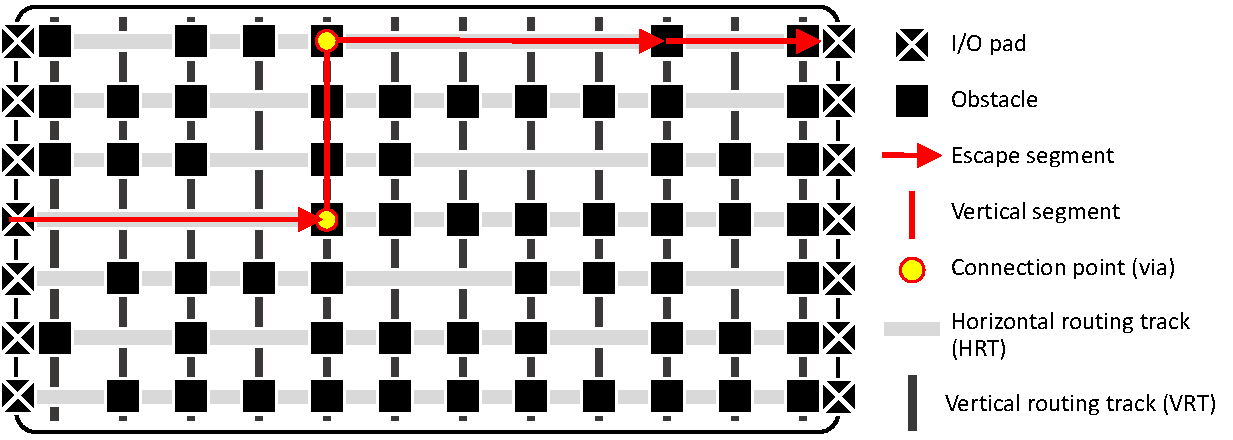
\includegraphics[width=1\linewidth]{figures/SneakySnake-Figure1.pdf}}
\caption{\alser{{Chip layout with processing elements and two layers of metal routing tracks. In this example, the chip layout has 7 horizontal routing tracks (HRTs) located on the first layer and another 12 vertical routing tracks (VRTs) located on the second layer. 
%We show only a single VRT out of the 12 VRTs for simplicity of illustration. 
The optimal signal net that is calculated using the SneakySnake algorithm 
%(the solution to the single net routing problem) 
is highlighted in red using three escape segments. The first escape segment is connected to the second escape segment using {a} VRT through vias. The second escape segment is connected to the third escape segment without passing through a VRT as both escape segments are located on the same HRT. The optimal signal net passes through three {obstacles (each of which is located at the end of each escape segment)} and hence the signal net has a total delay of} $3\times t_{obstacle}$.}}
\label{fig:overview}
\end{figure}

\begin{itemize}
%\item The chip layout has two layers of evenly spaced metal routing tracks. While the first layer allows traversing the chip horizontally through dedicated \emph{horizontal routing tracks} (HRTs), the second layer allows traversing the chip vertically using dedicated \emph{vertical routing tracks} (VRTs).

\item The chip layout has two layers of evenly spaced metal routing tracks. While the first layer allows traversing the chip horizontally through dedicated \emph{horizontal routing tracks} (HRTs), the second layer allows traversing the chip vertically using dedicated \emph{vertical routing tracks} (VRTs).

\item The horizontal and vertical routing tracks induce a two dimensional uniform grid over the chip layout. Each HRT can be obstructed by some obstacles (e.g., processing elements in the chip). \alser{For simplicity, we assume that VRTs can not be obstructed by obstacles.} These obstacles allow the signal to pass horizontally through HRTs, but they induce a signal delay on the passed signal. Each obstacle induces a fixed propagation delay, $t_{obstacle}$, on the victim signal that passes through the obstacle in the corresponding HRT.
\item A signal net often uses a sequence of alternating horizontal and vertical segments that are parts of the routing tracks. Adjacent horizontal and vertical segments in the signal net are connected by an inter-layer \emph{via}. \alser{We call a signal net \emph{optimal} if it is both the shortest and the fastest routing path 
(i.e., passes through the minimum number of obstacles)}.
\item \alser{Alternating between horizontal and vertical segments is restricted by passing a single obstacle. Thus, segment alternating strictly} delays the signal by $t_{obstacle}$ time.
\item The terminals can be any of the I/O pads that are located on the right-hand and left-hand boundaries of the chip layout. The source terminal always lies on the opposite side of the destination terminal.
\end{itemize}

The general goal of this SNR problem is to find an \emph{optimal} signal net in the grid graph of the chip layout. 
For the simplicity of developing a solution, we call a horizontal segment that ends with at most an obstacle an \emph{escape segment}. 
The escape segment can also be a single obstacle only. Also for simplicity, we call the right-hand side of an escape segment {a} \emph{checkpoint}. 
%We relax this definition later in Section \ref{Snake-on-Chip-Section} to allow partitioning the single net routing problem into smaller subproblems that can be solved independently and in parallel. 
Next, we present how we can reduce the ASM problem to the SNR problem.

\subsection{Reducing the Approximate String Matching (ASM) Problem to the Single Net Routing (SNR) Problem}\label{ASM2SNR}
%Our goal is to reduce the time calculate the sequence alignment accurately and quickly. 
%There are two challenges \alser{against} improving today's sequence alignment algorithms that we need to tackle. 
%(1) How to build a data structure that is simpler than the DP table \alser{(i.e., \emph{data-dependency free})} and yet \alser{it} accurately represents the similarities and the differences between two sequences. 
%(2) How to compute the \emph{optimal} number of differences between the two sequences using this new data structure. 
%To this end, w
We reduce the problem of finding the similarities and differences between two genomic sequences to that of finding the optimal signal net in a VLSI chip layout.
\alser{Reducing the ASM problem to the SNR problem requires two key steps: (1) replacing the DP table used by \alser{the} sequence alignment algorithm \alser{to} a special grid graph called \emph{chip maze} and (2) finding the number of differences between two genomic sequences} \unskip\parfillskip 0pt \par

\begin{figure*}
\centerline{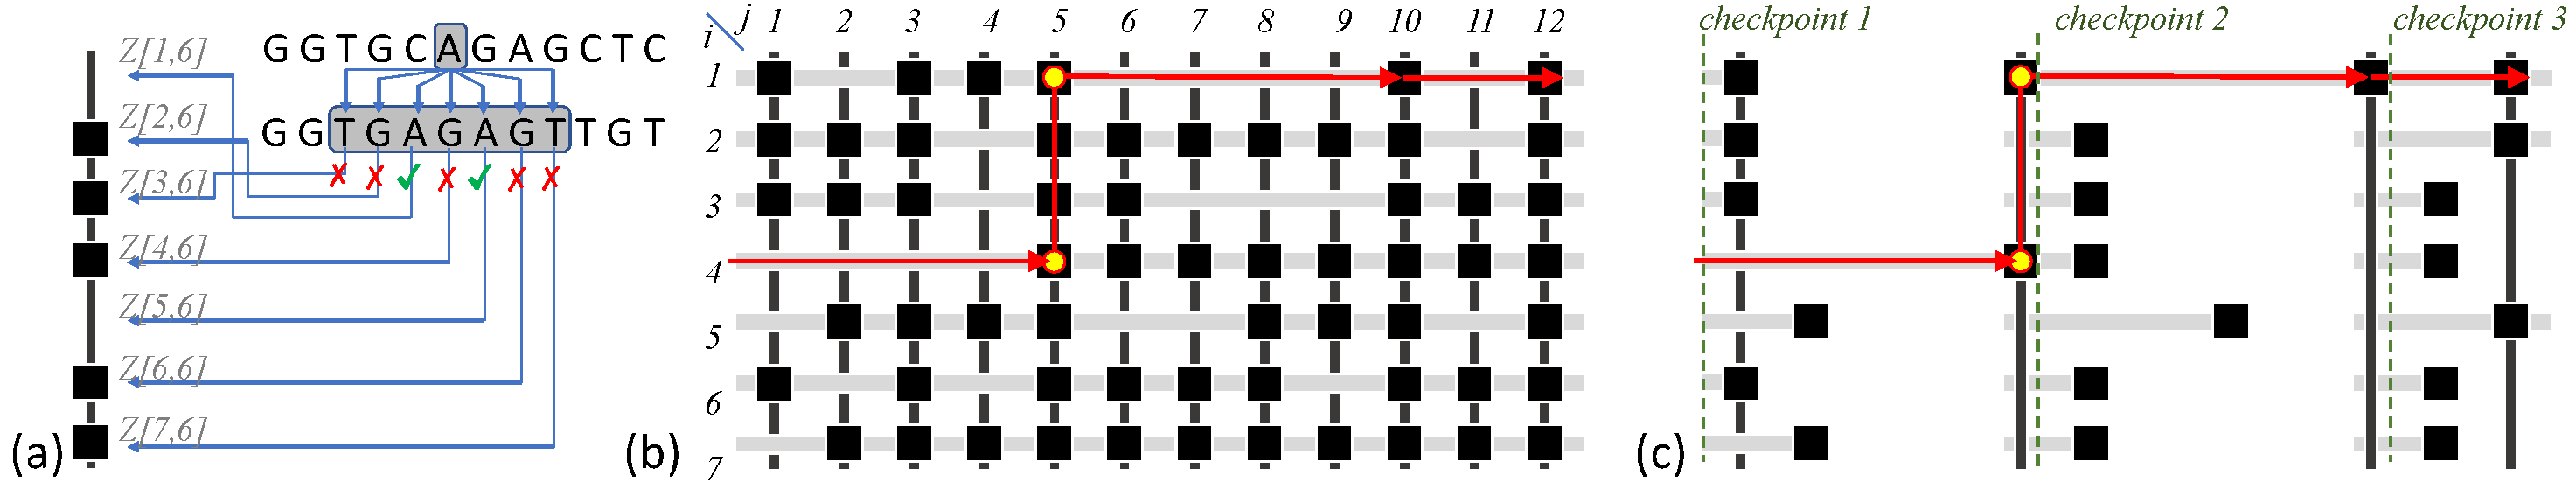
\includegraphics[width=0.95\linewidth]{figures/SneakySnake-Figure2.pdf}}
\caption{{(a) An example of how we build the 6$^{th}$ column of the chip maze, $Z$, using Equation 1 for \alser{a reference sequence} $R$ = \lq{GGTGCAGAGCTC}\rq{}, \alser{a query sequence} $Q$ = \lq{GGTGAGAGTTGT}\rq{}, and an edit distance threshold ($E$) of 3. The 6$^{th}$ character of $R$ is compared with each of its corresponding $2E+1$ characters of $Q$. 
{The order of the results of comparing $R[6]$ with $Q[3]$, $Q[4]$, and $Q[5]$ is reversed to easily derive the second case of Equation 1}.
(b) The complete chip maze that is calculated using Equation 1, which has 2$E$+1 rows and $m$ (length of $Q$) columns. (c) The actual chip maze that is calculated using the SneakySnake algorithm. The optimal signal net is highlighted in both chip mazes in red. The signal net has 3 obstacles {(each of which is located at the end of each escape segment)} and hence sequence alignment is needed, as the number of differences $\leq E$.}}
\label{fig:steps}
\end{figure*}

\noindent \alser{in the chip maze by solving the SNR problem.} 
We replace the $(m+1) \times (m+1)$ DP table with our chip maze, $Z$, where $m$ is the sequence length (for simplicity, we assume that we have a pair of equal-length sequences but we relax this assumption in {Section}~\ref{theorem}). 
The chip maze is a $(2E+1) \times m$ grid graph, where $E$ is the edit distance threshold {in terms of {the number of} tolerable character differences}, $(2E+1)$ is the number of HRTs, and $m$ is the number of VRTs. 
The chip maze is an abstract layout for the VLSI chip layout, \alser{as we show in Fig. \ref{fig:steps}(b) for the same chip layout of Fig. \ref{fig:overview}}. 
Each entry of the chip maze represents the pairwise comparison result of a character of one sequence with another character of the other sequence. 
A pairwise mismatch is represented by an obstacle (an entry of value '1') in the chip maze and a pairwise match is represented by an available path (an entry of value '0') in its corresponding HRT.
Given two genomic sequences, a reference sequence $R[1\dots m]$ and a query sequence $Q[1\dots m]$, and an edit distance threshold $E$, we calculate the entry $Z[i, j]$ of the chip maze, where $1\leq i\leq (2E+1)$ and $1\leq j\leq m$, as follows:\newline
\begin{equation}
\label{equ:chipmaze}
Z[i,j]=\left\{\begin{matrix*}[l]
0,\quad\quad if~~i=E+1, ~Q[j]=R[j],  \\ 
0,\quad\quad if~~1\leq i\leq E, ~Q[j-i]=R[j],  \\ 
0,\quad\quad if~~i> E+1, ~Q[j+i-E-1]=R[j],  \\ 
1,\quad\quad otherwise 
\end{matrix*}\right.
\end{equation}

We derive {the four cases of Equation 1} by considering  all possible pairwise matches and mismatches (due to possible edits) between two sequences. That is, each column of the chip maze stores the result of comparing the $j^{th}$ character of the \alser{reference sequence}, $R$, with each of {the} corresponding $2E+1$ characters of the \alser{query sequence}, $Q${, as we show in Fig.} \ref{fig:steps}(a). 
{In the first case of Equation 1, we compare the $j^{th}$ character of the reference sequence, $R$, with the $j^{th}$ character of the query sequence, $Q$, to detect pairwise matches and substitutions.
In the second case of Equation 1, we compare the $j^{th}$ character of the reference sequence with each of the $E$ left-hand neighboring characters of the $j^{th}$ character of the query sequence, to accurately detect deleted characters in the query {sequence}.
In the third case of Equation 1, we compare the $j^{th}$ character of the reference sequence with each of the $E$ right-hand neighboring characters of the $j^{th}$ character of the query sequence, to accurately detect inserted characters in the query {sequence}}. 
Each insertion and deletion can shift multiple trailing characters (e.g., deleting the character \lq{N}\rq{} from \lq{GE\textbf{N}OME}\rq{} shifts the last three characters to the left direction, making it \lq{GE\textbf{OME}}\rq{}). {Hence, in the second and the third cases of Equation 1,} we need to compare a character of the \alser{reference sequence} with the neighboring characters of its corresponding character of the \alser{query sequence} to cancel the effect of deletion/insertion and correctly detect the common subsequences between two sequences. 
%have no shift effect on the alignment of subsequent bases, comparing the $j^{th}$ character of the \alser{reference sequence}, $R$, with the $j^{th}$ character of the \alser{query sequence}, $Q$, is needed to find such substitutions.
%these $2E+1$ characters of the \alser{query sequence}, $Q$, are as follows: the $j^{th}$ character of the \alser{query sequence} {(case 1)}, the $E$ right-hand neighboring characters of the $j^{th}$ character, and the $E$ left-hand neighboring characters of the $j^{th}$ character. 
%Each insertion and deletion can shift multiple trailing characters (e.g., deleting the character \lq{N}\rq{} from \lq{GE\textbf{N}OME}\rq{} shifts the last three characters to the left direction, making it \lq{GE\textbf{OME}}\rq{}). Hence, we need to compare a character of the \alser{reference sequence}, $R$, with the neighboring characters of its corresponding character of the \alser{query sequence}, $Q$, to cancel the effect of deletion/insertion and correctly detect the common subsequences between two sequences. 
{In the fourth case of Equation 1,} we fill the remaining empty entries of each row {with} ones (i.e., obstacles) to indicate that there is no match between the corresponding characters.
{These four cases are essential to accurately detect} substituted, deleted, and inserted characters in one or both {of the} sequences. 
We present in Fig. \ref{fig:steps}(b) an example of the chip maze for two sequences, where a \alser{query sequence}, $Q$, differs from a \alser{reference sequence}, $R$, by three edits. 

The chip maze is a data-dependency free data structure as computing each of its entries is independent of every other and thus the entire grid graph can be computed all at once in a parallel fashion. Hence, our chip maze is well suited for both sequential and highly-parallel computing platforms \citep{seshadri2017ambit}.
%By building the chip maze, we address the first challenge against improving today's sequence alignment algorithms.
The challenge is now calculating the minimum number of edits between two sequences using the chip maze. 
Considering the chip maze as a chip layout where the rows represent the HRTs and the columns represent the VRTs, we observe that we can reduce the ASM problem to the SNR problem. 
Now, the problem becomes finding an optimal set (i.e., signal net) of non-overlapping escape segments. As we discuss in Section \ref{SNR_problem}, a set of escape segments is optimal if there is no other set that solves the SNR problem and has both {smaller} number of escape segments and {smaller} number of entries of value '1' (i.e., obstacles). Once we find such an optimal set \alser{of escape segments}, we can compute the minimum number of edits between two sequences as the total number of obstacles along the computed optimal set. 
Next, we present an efficient algorithm that solves this SNR problem.

%As an entry of value 0 in the chip maze represents a pairwise match, a sequence of horizontally consecutive entries of '0's forms a common subsequence between two sequences. 

%A set of one or more non-overlapping sequences of horizontally consecutive white shaded entries forms a sequence of pairwise matches. 
%If there is more than one sequence in this set, then there should be a black shaded entry that is located at the end of each sequence of consecutive white shaded entries (except probably the last sequence). 
%Hence, similar to the SNR problem, we call each sequence of consecutive white shaded entries including at most a single black shaded entry that is located right after the sequence as an escape segment. 
%These escape segments should also be non-overlapping as each entry indicates that the corresponding characters of both sequences are either similar or dissimilar. 
%The more the total number of these white shaded entries in a set the less the total number of black shaded entries. 




\subsection{Solving the Single Net Routing Problem}\label{theorem}
\alser{The primary purpose of the SneakySnake algorithm is to solve the SNR problem by providing an optimal signal net. 
Solving the SNR problem requires achieving two key objectives: 1) achieving the lowest possible latency by finding the minimum number of escape segments that are sufficient to link the source terminal to the destination terminal and 2) achieving the shortest length of the signal net by considering each escape segment just once and in monotonically increasing order of their start index (or end index). 
The first objective is based on a key observation that a signal net with fewer escape segments always {has} fewer obstacles, as each escape segment has at most a single obstacle (based on our definition in Section \ref{SNR_problem}). This key observation leads to a signal net that has the least possible total propagation delay. The second objective restricts the SneakySnake algorithm from ever searching backward for the longest escape segment. This leads to a signal net that has non-overlapping escape segments.

To achieve these two key objectives, the SneakySnake algorithm applies five effective steps. (1) The SneakySnake algorithm first constructs the chip maze {using Equation 1}. 
It then considers the first column of the chip maze as the first checkpoint, where the first iteration starts.
(2) At each new checkpoint, the SneakySnake algorithm always selects the longest escape segment that allows the signal to travel as far forward as possible until it reaches an obstacle. 
For each row of the chip maze, it computes the length of the first horizontal segment of consecutive entries of value '0' that starts from a checkpoint and ends at an obstacle or at the end of the current row. 
The SneakySnake algorithm compares the length of all the $2E+1$ computed horizontal segments, selects the longest one, and considers it along with its first following obstacle as an escape segment. 
If the SneakySnake algorithm is unable to find a horizontal segment (i.e., following a checkpoint, all rows start with an obstacle), it considers one of the obstacles as the longest escape segment. 
It considers the computed escape segment as part of the solution to the SNR problem. 
(3) It creates a new checkpoint after the longest escape segment. 
(4) It repeats the second and third steps until either the signal net reaches a destination terminal, or the total propagation delay exceeds the allowed propagation delay threshold (i.e., $E\times t_{obstacle}$).} 
{When the two input sequences are different in length, {we} need to count the number of obstacles more conservatively along {the signal net}. 
Doing so ensures a correct reduction of the ASM problem. 
This means that we need to deduct the total number of leading and trailing obstacles from the total count of edits between two input sequences before making the filtering decision, as such obstacles can be caused by the fourth case of Equation 1.} 
(5) If SneakySnake finds the optimal net using the previous steps, then {it indicates that the edit distance between two input sequences is $\leq E$}.
{If so, sequence alignment is needed to know the exact number of edits, type of each edit, and location of each edit between the two} sequences using user's favourite sequence alignment algorithm. 
Otherwise, the SneakySnake algorithm terminates without performing computationally expensive sequence alignment{, since the differences between sequences is guaranteed to be $>E$}.
%For the rest of the paper, we consider examining only a pair of equal-length input sequences as the general case since it is more challenging and includes more computations, as it examines the similarity end-to-end.

To efficiently implement the SneakySnake algorithm, we use an implicit representation of the chip maze. That is, the SneakySnake algorithm starts computing on-the-fly one entry of the chip maze after another for each row until it faces an obstacle (i.e., $Z$[$i$,$j$] = 1) or it reaches the end of the current row. 
Thus, the entries that are actually calculated for each row of the chip maze are the entries that are located only between each checkpoint and the first obstacle, in each row, following this checkpoint, as we show in Fig. \ref{fig:steps}(c). 
This significantly reduces the number of computations needed for the SneakySnake algorithm.
We provide the SneakySnake algorithm along with analysis of its computational complexity (asymptotic run time and space complexity) in \textcolor{black}{Supplementary Materials, Section 5}.

The SneakySnake algorithm is both correct and optimal {in solving the SNR problem}. 
The SneakySnake algorithm is correct as it always provides a signal net (if it exists) that interconnects the source terminal and the destination terminal. 
In other words, it does not lead to routing failure as signal will eventually reach its destination.

\textbf{Theorem 1.} \emph{The SneakySnake algorithm {is guaranteed} to find a signal net that interconnects the source terminal and the destination terminal when one exists.\\}
We provide the correctness proof for Theorem 1 in \textcolor{black}{Supplementary Materials, Section 6.1}. 
The SneakySnake algorithm is also optimal as it {is guaranteed} to find an optimal signal net that links the source terminal to destination terminal when one exists. 
Such an optimal signal net always ensures that the signal arrives the destination terminal with the least possible total propagation delay.

\textbf{Theorem 2.} \emph{When a signal net exists between the source terminal and the destination terminal, using the SneakySnake algorithm, a signal from the source terminal reaches the destination terminal with the minimum possible latency.\\}
We provide the optimality proof for Theorem 2 in \textcolor{black}{Supplementary Materials, Section 6.2}.
%Unlike existing sequence alignment algorithms that are based on DP~\citep{daily2016parasail} or sparse DP~\citep{chaisson2012mapping, schmidt2019accurate} approaches, SneakySnake has three unique advantages that we discuss in Supplementary Materials, Section 8.
\\\vspace{-10 pt}

{\textbf{Different from existing sequence alignment algorithms} that are based on DP approaches} \citep{daily2016parasail, xin2013accelerating} or sparse DP (i.e., chaining exact matches between two sequences using DP algorithms) approaches \citep{chaisson2012mapping}, 
%schmidt2019accurate}, 
{SneakySnake 1) does not require knowing the location and the length of {common subsequences} between the two {input} sequences in advance, 2) does not consider the vertical distance (i.e., the number of rows) between two escape segments in the calculation of the minimum number of edits, and 3) does not build the entire dynamic programming table; SneakySnake builds only a minimal portion of the chip maze that is needed to provide an optimal solution.
The first difference makes SneakySnake independent of any algorithm that aims to calculate sequence alignment, as SneakySnake quickly and efficiently calculates its own data structure (i.e., chip maze) to find \emph{all} {common subsequences}. {The second difference helps {to construct} a data dependency-free chip maze and allows for solving many SNR subproblems in parallel as calculating the routing path after facing an obstacle is independent of the calculated path before this obstacle.}
%simplifies the computations of SneakySnake but tends to underestimate the actual number of edits between two sequences. Slightly underestimating the number of edits while achieving fast computation is acceptable as long as we do not overestimate the number of edits. 
The third difference significantly reduces the number of computations needed for the SneakySnake algorithm.}

%The first difference makes SneakySnake independent of any algorithm that aims to calculate sequence alignment, as SneakySnake quickly and efficiently calculates its own data structure (i.e., chip maze) to find \emph{all} exact matches.
%The second difference simplifies the computations of SneakySnake but tends to underestimate the actual number of edits between two sequences. 
%To fix this issue, we need to consider the number of obstacles of the vertical segment that links each two adjacent escape segments in the calculation of the number of edits. 
%We need to enumerate all possible combinations of vertical segments and escape segments that exist after each escape segment and select the one that provides the least number of obstacles.
%This enforces us to use a DP table to avoid re-computing the length of the same escape segments many times unnecessarily. In fact, we avoid using DP tables to achieve fast and parallel calculation of the optimal signal net. 
%Slightly underestimating the number of edits while achieving fast computation is acceptable as long as we do not overestimate the number of edits.

\textbf{Different from existing edit distance approximation algorithms} \citep{chakraborty2018approximating,charikar2018estimating}
%\citep{batu2006oblivious,andoni2012approximating,chakraborty2018approximating,charikar2018estimating}
that sacrifice the optimality of the edit distance solution (i.e., its solution $\geq$ the actual edit distance of each sequence pair) for a reduction in time complexity, (e.g., $O(m^{1.647})$ instead of $O(m^{2})$), SneakySnake does not overestimate the edit distance as the calculated optimal signal net has \emph{always} the minimum possible number of obstacles (Theorem 2).
{We {take advantage of} the edit distance underestimation of SneakySnake by using our fast computation method as a pre-alignment filter}.
%ing step to decide whether {or not} sequence alignment computation is needed. 
%If two sequences have more edits than the edit distance threshold, $E$, then we do \emph{not} need computationally costly algorithms to conclude that the two sequences have unacceptable number of edits. But if the number of edits is less than or equal the edit distance threshold, then our filtering step should be followed by accurate sequence alignment algorithms, where users can choose different scoring functions. 
{Doing so} {ensures} two key properties: \alser{(1) {allows} sequence alignment to be calculated only for similar (or nearly similar) sequences and (2) {accelerates} the sequence alignment algorithms without changing (or replacing) their algorithmic method and hence preserving all the capabilities of the sequence alignment algorithms}.

%We observe that the backtracking step of a global alignment algorithm finds the optimal sequence of edit operations between two sequences by examining the value of the entries from the bottom-right entry of the DP table to the top-left entry. Similar to a global alignment algorithm, the first escape segment in the optimal solution set should start from any entry of the first column of the chip maze. Similarly, the last escape segment in the set should end at any entry of the last column of the chip maze. 

%Until now, we explain how SneakySnake examines a pair of equal-length input sequences. When the two input sequences are different in length, then we need to count the number of obstacles more conservatively along the optimal solution set. 
%Doing so ensures a correct reduction of the ASM problem. 
%Sequence alignment can be performed as a \emph{global} alignment, where two sequences of the same length are aligned end-to-end, or a \emph{local} alignment, where subsequences of the two given sequences are aligned. It can also be performed as a \emph{semi-global} alignment, where the entirety of one sequence is aligned to one of the ends of the other sequence. 
%This means that we need to deduct the total number of leading and trailing obstacles from the total count of edits between two {input} sequences before making the filtering decision. 
%Similarly for a semi-global alignment, we should not consider the leading or the trailing obstacles. 
%For the rest of the paper, we consider only the global alignment as the general case since it is more challenging and includes more computations, as it examines the similarity end-to-end.



%\alser{Next, we discuss an efficient implementation of the SneakySnake algorithm. Instead of building the chip maze explicitly, we use an implicit representation of the chip layout. That is, we compute each row of the chip maze \emph{on-the-fly}. The computation of the chip maze consists of two steps: (1) gradually shifting the \alser{query sequence}, $Q$, and (2) performing pairwise comparison of the shifted version of $Q$ with the \alser{reference sequence}, $R$. The SneakySnake algorithm shifts the \alser{query sequence} by $r$ steps to construct the $r^{th}$ row that is located above or below the $E+1^{th}$ row (called main diagonal in Fig. \ref{fig:steps}(d)) of the chip maze, where $1\leq r\leq E$. The shift direction is performed in the right-hand direction if the row is located above the $E+1^{th}$ row of the chip maze. Otherwise, the shift direction is performed in the left-hand direction. At each checkpoint, the SneakySnake algorithm starts computing on-the-fly one entry after another for each row until it faces an obstacle (the character of $Q$ at the current index mismatches its corresponding character of $R$) or it reaches the end of the row. Thus, the entries that are actually calculated for each row of the chip maze are the entries that are located only between each checkpoint and the first obstacle, in each row, following this checkpoint. This significantly reduces the number of computations needed for the SneakySnake algorithm as we discuss in detail in \textcolor{black}{Supplementary Materials, Section 7}.} 

%It is important to notice that if the first and the last longest escape segments are longer than their corresponding escape segments that are located at the $E+1^{th}$ horizontal routing track, then we penalize each by an obstacle's worth of propagation delay (i.e., $t_{obstacle}$). This ensures to increase the accuracy of the SneakySnake algorithm to be as close as possible to that of a global alignment algorithm.
We next discuss further optimizations and new software/hardware co-designed versions of the SneakySnake algorithm that {can} leverage FPGA and GPU architectures for highly-parallel computation.\\ 

\subsection{Snake-on-Chip Hardware Architecture} \label{Snake-on-Chip-Section}
We introduce an FPGA-friendly architecture for the SneakySnake algorithm, called \emph{Snake-on-Chip}. The main idea behind the hardware architecture of Snake-on-Chip is to divide the SNR problem into smaller non-overlapping subproblems. Each subproblem has a width of $t$ VRTs and a height of $2E+1$ HRTs, where $1<t\leq m$. We then solve each subproblem independently from the other subproblems. This approach results in three key benefits. 
(1) Downsizing the search space into a reasonably small grid graph with a known dimension {at} design time limits the number of all possible solutions for that subproblem. This reduces the size of the look-up tables (LUTs) required to build the architecture and simplifies the overall design. 
(2) Dividing the SNR problem into subproblems helps to maintain a modular and scalable architecture that can be implemented for any sequence length and edit distance threshold. (3) All the smaller subproblems can be solved independently and rapidly {with} high parallelism. This reduces the execution time of the overall algorithm as the SneakySnake algorithm does not need to evaluate the entire chip maze. 

However, these three key benefits come at the cost of accuracy degradation. As we demonstrate in Theorem 2, the SneakySnake algorithm guarantees to find an optimal solution to the SNR problem. However, the solution for each subproblem is not necessarily part of the optimal solution for the main problem (with the original size of $(2E+1) \times m$). This is because the source and destination terminals of these subproblems are not necessarily the same. 
{The SneakySnake algorithm determines the source and destination terminals for each SNR subproblem based on the optimal signal net of each SNR subproblem.}
%The source and destination terminals should be located at any of the $2E+1$ entries of the first and the last VRTs, respectively, of each subproblem, but the SneakySnake algorithm determines the exact location of the source and destination terminals for each subproblem based on its individual optimal solution. 
This {leads to underestimation of} the total number of obstacles found along each signal net of each SNR subproblem. This is still acceptable as long as {the SneakySnake algorithm} solves the SNR problem quickly and {\emph{without}} {\emph{overestimating}} the number of obstacles {compared to the edit distance threshold}.
We provide the details of our hardware architecture of Snake-on-Chip in \textcolor{black}{Supplementary Materials, Section 8}.

%Next, we present the details of our hardware architecture of Snake-on-Chip in four key steps. \alser{(1) Snake-on-Chip constructs the \emph{entire} chip maze of each subproblem. Each chip maze has $2E+1$ bit-vectors (rows) and each bit-vector is $t$ bits long. This is now different from the CPU implementation of the SneakySnake algorithm, as the number of entries computed in each row is no longer limited to the entries that are located only between a checkpoint and the first following obstacle. 
%This is due to the fundamental difference between CPU core (sequential execution) and FPGA chip (parallel processing).
%We want to concurrently compute all bits of all bit-vectors beforehand so that we can exploit massive bitwise parallelism provided by FPGA and perform computations on all bit-vectors in a parallel fashion. 

%(2) It computes the length of the first horizontal segment of consecutive zeros for each bit-vector (i.e., each HRT) using a leading-zero counter (LZC). Snake-on-Chip uses the LZC design proposed in \citep{dimitrakopoulos2008low} as it requires low number of both logic gates and logic levels. It counts the number of consecutive zeros that appear in a $t$-bit input vector before the first more significant bit that is equal to one. 
%The $t$-LZC generates two output signals, a $C$ bit-vector and a $Valid$ flag, for an input word $A = A_{t-1}, A_{t-2}, \dots, A_0$, where $A_{t-1}$ is the most significant bit. Only when all input bits are set to zero, the $Valid$ flag is set to one. 
%For other values of input $A$, the $C$ bit-vector represents the number of leading zeros in binary. The $C$ bit-vector encodes $log_2 t$ bits. The LZC sets $C_0$ to one if its leading-zero count is an odd number. Otherwise, it is set to zero. 
%For the case of an 8-bit input operand ($t$ = 8 bits), the two output signals of the LZC are given by:
%\begin{equation} 
%\begin{aligned}
%\overline{C_2} & = A_7 + A_6 + A_5 + A_4 \\
%\overline{C_1} & = A_7 + A_6 + \overline{A_5} \cdot  %\overline{A_4} \cdot (A_3+A_2)  \\
%\overline{C_0} & = A_7 + \overline{A_6} \cdot A_5 + %\overline{A_6} \cdot \overline{A_4} \cdot A_3 + %\overline{A_6} \cdot \overline{A_4} \cdot %\overline{A_2} \cdot A_1 \\
%\overline{Valid} &= A_7 + A_6 + A_5 + A_4 + A_3 + A_2 + A_1 + A_0
%\end{aligned}
%\end{equation}

%(3) Snake-on-Chip finds the bit-vector (i.e., HRT) that has the largest number of leading zeros. Snake-on-Chip implements a hierarchical comparator structure with $\ceil{log_2(2E+1)}$ levels. Each comparator compares the output of two LZCs and finds the largest value. That is, we need $2E+2$ comparators, each of which is a $(\floor{log_2t}+1)$-bit comparator, for comparing the leading zero counts of $2E+1$ $t$-bit LZCs and finding the largest leading zero count. 
%We provide in Fig. \ref{fig:comp} the proposed architecture of the 4-bit LZC comparator. 
%\begin{figure}
%\centerline{\includegraphics[width=\linewidth]{figures/SS-fig3.pdf}}
%\caption{Proposed 4-bit LZC comparator.}
%\label{fig:comp}
%\end{figure}
%It simply checks if at least one of the two input $Valid$ signals is set to zero (meaning that one of the two escape segments is 8-bit long), then it sets the output of the LZC comparator, $Valid$ and $C$ bit-vector, all to zero. Otherwise, if both input $Valid$ signals of both relevant LZCs are set to 1, then the LZC comparator compares the $C$ bit-vector of the first LZC with the $C$ bit-vector of the second LZC. It selects the $C$ bit-vector that has the largest value and passes it to its output $C$ bit-vector along with a $Valid$ signal of value one.
%\begin{figure*}
%\centerline{\includegraphics[scale=0.2]{figures/SS-fig4.pdf}}
%\caption{Block diagram of the 11 LZCs and the hierarchical LZC comparator tree for computing the largest number of leading zeros in 11 rows.}
%\label{fig:LZC}
%\end{figure*}
%Consider that we choose $t$, $E$, and $m$ to be 8 columns, 5 edits (i.e., 11 rows), and 100 characters, respectively. This results in partitioning the chip maze of size 11 $\times$ 100 into 13 subproblems, each of size 11 $\times$ 8. We need 11 LZCs and 12 comparators. 
%We arrange the 12 comparators into 4 hierarchical levels: the first level that is closer to the LZCs has 6 comparators, the second level has 3 comparators, the third level has 2 comparators, and the last level has a single comparators.
%This hierarchical comparator structure compares the 11 escape segments of a subproblem and produces a $Valid$ signal and a $C$ bit-vector that contains information about the length of the longest segment of consecutive zeros. 
%We provide a block diagram of the 4-level LZC comparator tree including the 11 LZCs in} \textcolor{black}{Supplementary Materials, Fig. 10}. 

%(4) After computing the length of the longest segment (the largest leading-zero count), Snake-on-Chip creates a new checkpoint in order to iterate over the HRTs once again to find the next optimal escape segment.
%Snake-on-Chip achieves this by shifting the bits of each row (i.e., HRT) to the right-hand direction (assuming the least significant bit starts from the right-hand side). The shift amount is equal to $x$ bits, where $x$ is the length of the previously-found longest escape segment of the consecutive zeros.
%To skip the obstacle that exists at the end of the longest escape segment, Snake-on-Chip shifts the bits of each row by an additional single step to the right-hand direction. This guarantees to exclude the previously-found longest escape segment along with a single obstacle from the new search round.

%(5) As now, Snake-on-Chip preprocesses all the $2E+1$ rows and make them ready for the next search round. Snake-on-Chip repeats the previous four steps in order to find the next optimal escape segment starting from the least significant bit all the way to the most significant bit. Repeating the previous steps for each iteration requires building a new replication for the architecture design of all the four previous steps. The number of replications needed depends on the desired accuracy of the SneakySnake algorithm. If our target is to find an optimal signal net that has at most a single obstacle within each subproblem, then we need to build two replications for the three previous steps (steps 2, 3, and 4). For example, let $A$ be \lq{00010000}\rq{}, where $t = 8$. The first replication computes the value of $x$ as four zeros and updates the bits of $A$ to \lq{11111000}\rq{}. The second replication computes the value of $x$ as three zeros and updates the bits of $A$ to \lq{11111111}\rq{}. 

%(6) The last step is to calculate the total number of obstacles faced along the entire optimal signal net in each subproblem. For each subproblem, Snake-on-Chip calculates the total number of obstacles as follows:
%\begin{equation} 
%min⁡(y,t-\sum_{k=1}^{y} x_k)
%\end{equation}
%where $y$ is the total number of replications included in the architecture of Snake-on-Chip and $x_k$ is the length of the longest segment of consecutive zeros found by the replication of index $k$. Hence, the total number of obstacles for the original problem of size $(2E+1) \times m$ is simply the summation of the total number of obstacles faced along the optimal signal net of all subproblems.


\subsection{Snake-on-GPU Parallel Implementation} \label{Snake-on-GPU-Section}
%This section is prepared by Juan
{We} introduce our GPU implementation of the SneakySnake algorithm, called \emph{Snake-on-GPU}.
The main idea of Snake-on-GPU is to exploit the large number (typically few thousands) of GPU threads provided by modern GPUs to solve a large number of SNR problems rapidly and concurrently. 
In Snake-on-Chip, we explicitly divide the SNR problem into smaller non-overlapping subproblems and then solve all subproblems concurrently and independently using our specialized hardware. 
In Snake-on-GPU, we follow a different approach than that of Snake-on-Chip by keeping the same size of the original SNR problem and solving a massive number of these SNR problems at the same time. %(depending on the available number of GPU threads [\textcolor{black}{JGL: This makes no sense. The limitation in the number of SNR problems that you can solved is not related to the number of GPU threads. In two different GPUs, you can solve the same number of problems -> rephrase: granularity that fits best}]) 
%[\textcolor{black}{JUAN or TAHA please add reference if it is true -> It is not true and not a good sentence. It adds unnecessary confusion. We don't need to divide the SNR problem among multiple threads for an efficient GPU implementation, but this does not mean that doing it would be "very inefficient"}]. 
Snake-on-GPU uses one single GPU thread to solve one SNR problem (i.e., comparing one query sequence to one reference sequence at a time). 
This granularity of computation fits well the amount of resources (e.g., registers) that are available to each GPU thread and avoids the need for synchronizing several threads working on the same SNR problem. %GPUs offer more flexibility to the users to change the values of some input parameters of Snake-on-Chip without the need to build a new design as in FPGAs.
%This approach obviates the need for assigning many threads for the same SNR problem and then collecting partial solutions from these threads for a single SNR problem, which is very inefficient for GPU implementation and time consuming

%As such, we need to compare each of the query sequences to all available reference sequences to calculate their similarities. 
%The number of query and reference sequences will typically be in the order of hundreds of thousands. 
%For such a large number of similarity calculations, SneakySnake can benefit from the throughput-oriented, massively-parallel architecture of GPUs.
Given the large size of the sequence pair dataset that the GPU threads need to access, we carefully design Snake-on-GPU to efficiently 1) copy the input dataset of query and reference sequences into the GPU global memory, which is the off-chip DRAM memory of GPUs~\citep{cuda-guide} and it typically fits a few GB of data and 2) allow each thread to store its own query and reference sequences using the on-chip register file to avoid unnecessary accesses to the off-chip global memory. Each thread solves the complete SNR problem for a single query sequence and a single reference  sequence.
We provide the details of our parallel implementation of Snake-on-GPU in \textcolor{black}{Supplementary Materials, Section 9}.

%Snake-on-GPU makes three key assumptions that help with providing an efficient GPU implementation. (1) The entire input dataset of query and reference sequences fits into the GPU global memory, which is the off-chip DRAM memory of GPUs~\citep{cuda-guide} and it typically fits a few GB of data. (2) We copy the entire input dataset from the CPU main memory to the GPU global memory before the GPU kernel execution starts. This enables massively-parallel computation by making large number of input sequences available in the GPU global memory. (3) We copy back the pre-alignment filtering results from the GPU global memory to the CPU main memory \emph{only} after the GPU kernel completes the computation. %and if later stages of the alignment pipeline do \emph{not} run on the GPU.
%If the size of the input dataset exceeds the size of the GPU global memory, we divide the dataset into independent smaller datasets, each of which can fit the capacity of the GPU global memory. 
%This approach also helps to overlap the computation performed on one small dataset with the transfer of another small dataset between the CPU memory and GPU memory~\citep{gomezluna2012}. 

%Given the large size of the input dataset that the GPU threads need to access from the GPU global memory, we carefully design Snake-on-GPU to efficiently %(1) access the off-chip GPU global memory with its full bandwidth, and (2) use on-chip memories, such as registers and scratchpad memory, to store the query and reference sequences, which are  reused many times, and avoid unnecessary accesses to the off-chip global memory. %JGL: We are no longer using the scratchpad memory.
%\juan{use the on-chip register file to store the query and the reference sequences and avoid unnecessary accesses to the off-chip global memory.}
%[\textcolor{black}{WHY? -> Why what? We need to use registers and scratchpad to take advantage of data reuse, and avoid too many accesses to global memory.}]
%JGL: The current implementation does not have coalesced memory accesses. This means that the access to global memory is not done in the most efficient way. With respect to the performance, the way we are accessing memory might still be ok, because we have L1 cache.
%For an efficient access to the GPU global memory, we need to ensure that the memory accesses are \emph{coalesced}~\citep{cuda-guide}, i.e., consecutive threads access consecutive 4-byte words from the same cache line. 
%This way of serving each memory request provides the minimum number of memory transactions and, thus, it boosts the overall performance by reducing the memory access time. 
%Snake-on-GPU uses linear addressing for each GPU thread to read 4 bytes of the query and reference sequences, as we show in Fig.~\ref{fig:snake-on-gpu}.
%The workflow of Snake-on-GPU includes two key steps.%, \juan{as we show in Fig.~\ref{fig:snake-on-gpu}}. %\CA{These circled numbers look UGLY.}
%\begin{figure}
%\centerline{\includegraphics[width=0.7\linewidth]{figures/Snake-on-GPU-Visio.pdf}}
%\caption{Workflow of Snake-on-GPU. It includes three key steps: (1) loading reference sequences into the scratchpad memory, (2) loading the query sequences into registers, and (3) each thread solves a single SNR problem.}
%\caption{Workflow of Snake-on-GPU. It includes three key steps: (1) each GPU thread loads a reference sequences into registers, (2) the thread loads the query sequence into registers, and (3) the thread solves a single SNR problem. \jgl{It is necessary to modify this figure to have registers for the refs too. Also, add the numbers (1), (2), (3).}}
%\label{fig:snake-on-gpu}
%\end{figure}
%First ((1) in Fig.~\ref{fig:snake-on-gpu}), %Snake-on-GPU places the reference sequences in the on-chip scratchpad memory of each GPU core, which is a shared memory space for the threads running in a GPU core. 
%1) Each thread copies a single reference sequence and another single query sequence \juan{from global memory to the on-chip registers.}
%This enables all the threads to access the reference sequences efficiently without repeatedly transferring them from the global memory for each thread. 
%With coalesced global memory accesses, these threads collaborate on loading into the scratchpad as many reference sequences as they can fit.
%Second ((2) in Fig.~\ref{fig:snake-on-gpu}), %~\circled{2}, 
%Snake-on-GPU places the query sequences into registers. 
%\juan{each thread copies a query sequence from global memory to on-chip registers.}
%Assuming the maximum length of a query sequence is $m$ (i.e., the maximum number of VRTs), we need $2m$ bits to encode each character of the query sequence to a unique binary representation.
%Assuming the maximum length of a query (or reference) sequence is $m$ (i.e., the maximum number of VRTs), we need $2m$ bits to encode each character of the query (or reference) sequence to a unique binary representation. 
%\juan{Since the size of a register is 4 bytes (32 bits), each thread needs $R = \ceil{\frac{2m}{32}}$ registers to store an entire query/reference sequence. For example, for a maximum length of $m$ = 128, $R$ = 8. This way, 16 registers are enough to store both query and reference sequence. This number is much lower than the maximum of 256 registers that each thread can use in current NVIDIA GPUs. Thus, the resources of a GPU core are not exhausted and more threads can run concurrently.}
%\taha{If each thread loads 32 bytes (256 bits) from the GPU global memory, we need a group of $T = \ceil{\frac{2m}{32}}$ threads to load an entire query sequence with the length of $m$ in a way that each of them contains a complete read.} 
%Third~\circled{3}, each thread solves the complete SNR problem for a single query sequence (that is loaded by the thread in its own register) and a single reference sequence (that is stored in the scratchpad memory). Each GPU thread applies the same computation of the SneakySnake algorithm to solve the SNR problem. For fast calculation of the number of consecutive zeros in GPUs, we use CLZ() function [\textcolor{black}{CITE}] that is the fastest GPU implementation [\textcolor{black}{JUAN or TAHA: PLEASE CHECK THIS and maybe talk about other functions used? -> I'm not convinced there is a need for talking about the CLZ function. Each thread applies SneakySnake as is, afaik. Or is the CLZ function exclusive of the GPU implementation?}].
%Once the GPU threads complete solving the SNR problems for all the query sequences loaded in the registers and all the reference sequences loaded in the scratchpad memory, Snake-on-GPU repeats step~\circled{1} and then step~\circled{3} as many times as needed [\textcolor{black}{WHY NOT step 2 as well? -> Step (2) is reading the query. Once the query is loaded, the thread just keeps it forever and compares it to all references. We might better want to invert the order and make the reading of the query step (1).}].
%2) \juan{Each thread solves the complete SNR problem for a single query sequence and a single reference sequence. Each GPU thread applies the same computation of the SneakySnake algorithm to solve the SNR problem.} 

\section{Results} \label{sec:results}
%\textcolor{red}{We selected five implementations, each of which represents a certain category of existing algorithms: (1) an implementation of the Farrar’s algorithm in the Parasail library (hereafter: Parasail; commit 3d8b4ee; [24]), (2) the global alignment routine in the BWA-MEM algorithm (BWA-MEM global; commit b582816), (3) re-implementation of the BLAST X-drop DP algorithm found in NCBI BLAST+ package (version 2.2.31+), (4, 5) the Myers’ bit-parallel edit distance algorithms [26] in the edlib and the SeqAn libraries (edlib; commit 0c6fe0f; [36] and SeqAn ED; version 1.4.2; [37], respectively). To our knowledge, other tools and libraries for long-read alignment fall largely on one of these categories.}
{We} evaluate 1) filtering accuracy, 2) filtering time, and 3) benefits of combining our universal implementation of the SneakySnake algorithm with state-of-the-art aligners.
%, and (5) the benefits of combining SneakySnake and Snake-on-Chip with read mappers. 
We provide {a comprehensive treatment {of} all evaluation results in the {Supplementary Excel File} and {on the SneakySnake GitHub page}.
We compare the performance of SneakySnake, Snake-on-Chip, and Snake-on-GPU to {four} pre-alignment filters, Shouji~\citep{alser2019shouji}, MAGNET~\citep{alser2017magnet1}, GateKeeper~\citep{alser2017gatekeeper}, and SHD~\citep{xin2015shifted}. 
{We run the experiments that use multithreading and long sequences {on} a 2.3 GHz Intel Xeon Gold 5118 CPU with up to 48 threads and 192 GB RAM.} 
We run all other experiments {on} a 3.3 GHz Intel E3-1225 CPU with 32 GB RAM. We use a Xilinx Virtex 7 VC709 board \citep{guide2013virtex} to implement Snake-on-Chip and other existing accelerator architectures {(}Shouji, MAGNET, and GateKeeper). We build the FPGA design using Vivado 2015.4 in synthesizable Verilog. We use {an} NVIDIA GeForce RTX 2080Ti card \citep{guide2019Nvidia2080} with a global memory of 11 GB {GDDR6} to implement Snake-on-GPU. Both Snake-on-Chip and Snake-on-GPU are \emph{independent} of the specific FPGA and GPU platforms as they do not rely on any vendor-specific computing elements (e.g., intellectual property cores).
%\vspace{-10 pt}

\subsection{{Evaluated Datasets}} \label{sec:experiment}
Our experimental evaluation uses 4 different real datasets (\texttt{100bp\_1}, \texttt{100bp\_2}, \texttt{250bp\_1}, and \texttt{250bp\_2}) and 2 simulated datasets (\texttt{10Kbp} and \texttt{100Kbp}). 
Each real dataset contains 30 million real sequence pairs (text and query pairs). \texttt{100bp\_1} and \texttt{100bp\_2} have sequences of length 100 bp, while \texttt{250bp\_1} and \texttt{250bp\_2} have sequences of length 250 bp.
We generate {the} \texttt{10Kbp} dataset to have 100,000 sequence pairs, each of which is 10 Kbp long, while {the} \texttt{100Kbp} dataset has 74,687 sequence pairs, each of which is 100 Kbp long.
{Supplementary Materials, Section 10.1 provides the details of these datasets}.


%We have two key approaches to generate sequence pairs for testing the performance of pre-alignment filters: 1) using existing read mappers to find reference segments that might be similar or dissimilar to real reads, and 2) using available read simulators.
%These reference segments generated by read mappers are not necessarily reported in their output SAM file, as they are generated before applying DP-based pairwise alignment step to ensure that the edit distance of every generated pair is not necessarily within the edit distance threshold. 
%%The read simulators allow controlling the type of edits, the number of edits, and their distribution over a sequence. However, it is challenging to avoid any bias in setting up their different simulator parameters.
%%We follow the second option for two key reasons. 1) It is used in evaluating a state-of-the-art pre-alignment filter, Shouji and 2) we aim to avoid any bias that might be introduced by setting up many simulator parameters and ensure having sequence pairs with different type of edits, a wide range of number of edits, and real distribution of edit locations.
%We follow both approaches, as they are still widely-used in evaluating existing algorithms.
%Our experimental evaluation uses 4 different real datasets and 2 simulated datasets. 

%\textbf{Real datasets.} Each real dataset contains 30 million real sequence pairs (text and query pairs). 
%We obtain two different read sets, ERR240727\_1 and SRR826471\_1, of the whole human genome that include two different read lengths, 100 bp and 250 bp, respectively. 
%We download these two read sets from EMBL-ENA (https://www.ebi.ac.uk/ena). 
%We map each read set to the human reference genome (GRCh37) using mrFAST \citep{alkan2009personalized} mapper and observe all potential mapping locations of every read.
%We obtain the human reference genome from the 1000 Genomes Project \citep{1000GP2015}.
%Before mapping the reads, we disable the DP-based pairwise alignment algorithm of mrFAST mapper to obtain both aligned and unaligned sequences. 
%For each read set, we use two different maximum numbers of allowed edits (2 and 40 for $m$ =100 bp and 8 and 100 for $m$ = 250 bp) using the $e$ parameter of mrFAST to generate four real datasets in total. 
%%Each dataset contains the sequence pairs that are generated by mrFAST mapper before the read alignment step of mrFAST, such that we allow each dataset to contain both similar (i.e., having edits fewer than or equal to the edit distance threshold) and dissimilar (i.e., having more edits than the edit distance threshold) sequences over a wide range of edit distance thresholds. 
%We provide the details of these four datasets in the \textcolor{black}{Supplementary Materials, Section 11.1}. For the reader's convenience, we refer to these datasets as Set\_1, Set\_2, Set\_3, and Set\_4.

%{\textbf{Simulated datasets.} We generate two sets (we refer to them as Set\_5 and Set\_6) of long sequence pairs using PBSIM} \citep{ono2013pbsim}. {We choose this simulator as it provides pairs of two sequences, the original segment of the reference (not only the location as in some read simulators) and its simulated segment. This helps us to directly obtain sequence pairs that can be used for evaluating the performance of sequence aligners and pre-alignment filters. We use Human chromosome 1 (GRCh38.p13 assembly, downloaded from https://www.ncbi.nlm.nih.gov/nuccore/NC\_000001.11) sequence for the input reference sequence in PBSIM. We generate Set\_5 to have 100,000 sequence pairs, each of which is 10 Kbp long, at 30x genome coverage. Set\_6 has 74,687 sequence pairs, each of which is 100 Kbp long, at 30x genome coverage. For both sets (Set\_5 and Set\_6), we use the default error profile for the continuous long reads (CLR) in PBSIM.}

\subsection{Filtering Accuracy}\label{filtering_accuracy}
We evaluate the accuracy of {a} pre-alignment filter by computing its rate of falsely-accepted and falsely-rejected sequences before performing sequence alignment. The false accept rate is the ratio of the number of dissimilar sequences that are falsely accepted by the filter and the number of dissimilar sequences that are rejected by the sequence alignment algorithm. 
The false reject rate is the ratio of the number of similar sequences that are rejected by the filter and the number of similar sequences that are accepted by the sequence alignment algorithm. A reliable pre-alignment filter should always ensure both a 0\% false reject rate {to maintain the correctness of {the} genome analysis pipeline and an \emph{as-small-as-possible}} false accept rate  {to} maximize the number of dissimilar sequences that are eliminated {at low performance overhead}.

We first assess the false accept rate of SneakySnake, Shouji, MAGNET, GateKeeper, and SHD across different four real datasets and edit distance thresholds of $0\%-10\%$ of the sequence length. In Fig. \ref{fig:false-accept-rate}, 
we provide the false accept rate of each of the five filters.
%(we provide the exact values in \textcolor{red}{Supplementary Materials, Section 10.2}). 
We use Edlib to identify the ground{-}truth truly-accepted sequences for each edit distance threshold. Based on Fig. \ref{fig:false-accept-rate}, we make four key observations. 
(1) SneakySnake provides the lowest false accept rate compared to all the four state-of-the-art pre-alignment filters. 
SneakySnake provides up to 31412$\times$, 20603$\times$, and 64.1$\times$ less number of falsely-accepted sequences compared to GateKeeper/SHD (using \texttt{250bp\_2}, $E$= 10\%), Shouji (using \texttt{250bp\_2}, $E$= 10\%), and MAGNET (using \texttt{100bp\_1}, $E$= 1\%), respectively.
(2) MAGNET provides the second lowest false accept rate. It provides up to 25552$\times$ and 16760$\times$ less number of falsely-accepted sequences compared to GateKeeper/SHD (using \texttt{250bp\_2}, $E$= 10\%) and Shouji (using \texttt{250bp\_2}, $E$= 10\%), respectively.
(3) All five pre-alignment filters are less accurate in examining \texttt{100bp\_1} and \texttt{250bp\_1} than the other datasets, \texttt{100bp\_2} and \texttt{250bp\_2}. {This is expected as the actual number of edits of most of the sequence pairs in \texttt{100bp\_1} and \texttt{250bp\_1} datasets is very close to the edit distance threshold (Supplementary Materials, Table 4) and hence any underestimation in calculating the edit distance can lead to {falsely{-}accepted sequence pairs (i.e.,} estimated edit distance} $\leq E$).
(4) GateKeeper and SHD become ineffective for edit distance thresholds of greater than 8\% and 3\% for sequence lengths of 100 and 250 characters, respectively, as they accept all the input sequence pairs. 
This causes {a read mapper using} them to examine each sequence pair unnecessarily twice (i.e., once by GateKeeper or SHD and once by the sequence alignment algorithm).

Second, we {find that} SneakySnake {has} a 0\% false reject rate {(not plotted)}. {This observation is in accord with our theoretical proof of Theorem 2.}
It is also demonstrated in \citep{alser2019shouji} that Shouji and GateKeeper have a 0\% false reject rate, while MAGNET can falsely reject some similar sequence pairs.
%We also observe that MAGNET provides a very low false reject rate of less than 0.00045\% for $E>$ 3\% of the sequence length using Set\_1 and Set\_3.

We conclude that SneakySnake improves the accuracy of pre-alignment filtering by up to four orders of magnitude compared to the state-of-the-art pre-alignment filters. We also conclude that SneakySnake is the most effective pre-alignment filter, with a very low false accept rate and a 0\% false reject rate across a wide range of both edit distance thresholds and sequence lengths.
%\vspace{-10 pt}

\begin{figure}
\centerline{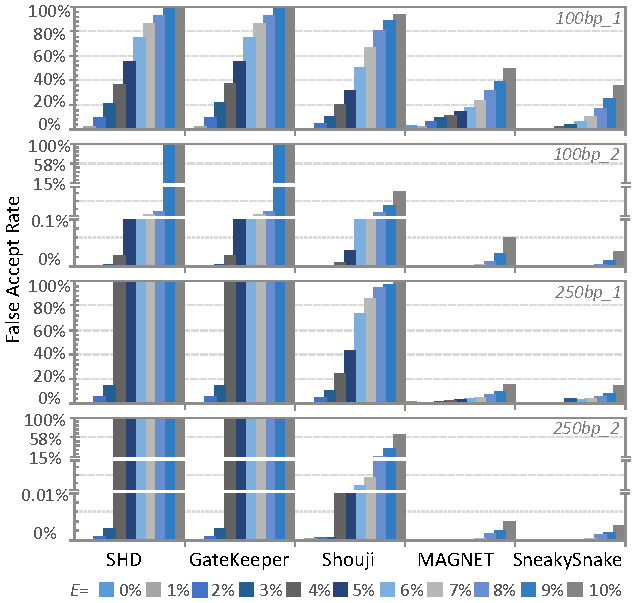
\includegraphics[width=1\linewidth]{figures/SS-fig5-false-accept-rate.pdf}}
\caption{{False accept rates of SHD, GateKeeper, Shouji, MAGNET, and SneakySnake across 4 real datasets of short sequences}. We use a wide range of edit distance thresholds ($0\%-10\%$ of the sequence length) for sequence lengths of 100 and 250 bp.}
\label{fig:false-accept-rate}
\end{figure}


\subsection{{Effect} of SneakySnake on Short Sequence Alignment}
We analyze the benefits of integrating CPU-based pre-alignment filters, SneakySnake and SHD with the state-of-the-art CPU-based sequence aligners, Edlib and Parasail. We evaluate all tools using a single CPU core and single thread environment. Fig. \ref{fig:CPUSneakySnake}(a) and (b) present the normalized end-to-end execution time of SneakySnake and SHD{,} each combined with Edlib and Parasail, using our four real datasets over edit distance thresholds of $0\%-10\%$ of the sequence length. We make four key observations. (1) The addition of SneakySnake as a pre-alignment filtering step {significantly} reduces the execution time of Edlib and Parasail by up to 37.7$\times$ (using \texttt{250bp\_2}, $E$= 0\%) and 43.9$\times$ (using \texttt{250bp\_2}, $E$ =2\%), respectively. 
We also observe a similar trend as the number of CPU threads increases from 1 to 40, as we {show} in Supplementary Materials, Section 10.2.
{To explore the reason for this significant speedup, we need to check how fast SneakySnake examines the sequence pairs compared to sequence alignment, which we observe next}.
(2) SneakySnake is up to 43$\times$ (using \texttt{250bp\_1}, $E$= 0\%) and  47.2$\times$ (using \texttt{250bp\_1}, $E$= 2\%) faster than Edlib and Parasail, respectively, in examining the sequence pairs. 
(3) SneakySnake provides up to 8.9$\times$ 
%(using Set\_4, $E$= 4\%) 
and 40$\times$ 
%(using Set\_4, $E$= 5\%) 
more speedup to the end-to-end execution time of Edlib and Parasail compared to SHD. This is expected as SHD produces a high false accept rate (as we show earlier in Section \ref{filtering_accuracy}).
(4) The addition of SHD as a pre-alignment step reduces the execution time of Edlib and Parasail for some of the edit distance thresholds by up to 17.2$\times$ (using \texttt{100bp\_2}, $E=0\%$) and 34.9$\times$ (using \texttt{250bp\_2}, $E$= 3\%), respectively. 
However, for most of the edit distance thresholds, we observe that Edlib and Parasail are faster alone than with SHD combined as a pre-alignment filtering step. This is expected as SHD becomes ineffective in filtering for $E$> 8\% and $E$> 3\% for $m$= 100 bp and $m$= 250 bp, respectively, (as we show earlier in Section \ref{filtering_accuracy}).

We conclude that SneakySnake is the best-performing CPU-based pre-alignment filter in terms of both speed and accuracy. Integrating SneakySnake with sequence alignment algorithms is always beneficial for short sequences and reduces the end-to-end execution time by up to an order of magnitude without the need for hardware accelerators. 
We also conclude that SneakySnake's performance {scales well} over a wide range of edit distance thresholds, number of CPU threads, and sequence lengths.


\begin{figure}
\centerline{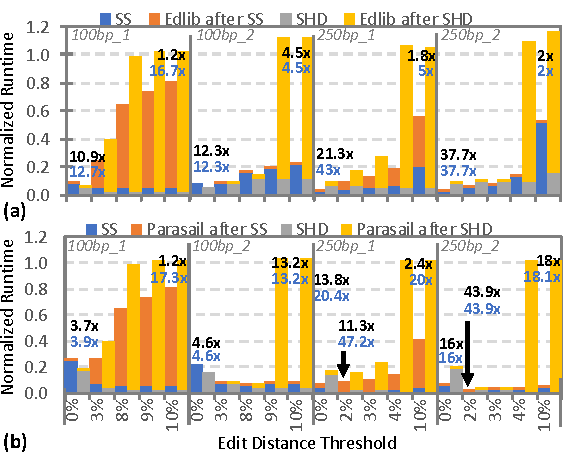
\includegraphics[width=1\columnwidth]{figures/Figure4-Oct2020.pdf}}
%\centerline{\includegraphics[width=0.8\textwidth]{figures/Figure4-March2020.pdf}}
\caption{\alser{Normalized end-to-end execution time of SneakySnake and SHD{, each} combined with (a) Edlib and (b) Parasail. 
{The execution time values in (a) and (b) are normalized to that of Edlib and Parasail, respectively, {without} pre-alignment filtering.}
We use four datasets over a wide range of edit distance thresholds ($E$= 0\%-10\% of the sequence length) for sequence lengths ($m$) of 100 bp {(\texttt{100bp\_1} and \texttt{100bp\_2})} and 250 bp {(\texttt{250bp\_1} and \texttt{250bp\_2})}.
We present two speedup {values} for $E$= 0\% and $E$= 10\% of {each dataset} and some other $E$ values highlighted by arrows. The {top} speedup {value} {(in black)} represents the end-to-end speedup that is gained from combining the pre-alignment filtering step with the alignment step. It is calculated as $A/(B+C)$, where $A$ is the execution time of the sequence aligner before adding SneakySnake {(not plotted in graphs)}, $B$ is the execution time of SneakySnake, and $C$ is the execution time of the sequence aligner after adding SneakySnake. The {bottom} speedup {value} {(in blue)} is calculated as $A/B$.% and it represents the speedup that is gained from using SneakySnake instead of the sequence alignment algorithm to examine all given sequence pairs.
}}
\label{fig:CPUSneakySnake}
\end{figure}

\subsection{{Effect} of Snake-on-Chip and Snake-on-GPU on Sequence Alignment}

We analyze the benefits of integrating Snake-on-Chip and Snake-on-GPU with the state-of-the-art sequence aligners, designed for different computing platforms in Fig. \ref{fig:Snake-on-Chip}.
{We} compare the effect of combining Snake-on-Chip and Snake-on-GPU with {an} existing sequence aligner {to} that of two state-of-the-art FPGA-based pre-alignment filters, Shouji and GateKeeper. 
We also select four state-of-the-art sequence aligners that are implemented for CPU (Edlib and Parasail), GPU (GSWABE), and FPGA (FPGASW). 
We use \texttt{100bp\_1} and \texttt{100bp\_2} in this {evaluation, as GSWABE, Shouji, and GateKeeper work for only short sequences}. GSWABE and FPGASW are not open-source and not available to us. Therefore, we scale {their} reported number of computed entries of the DP matrix {per} second (i.e., GCUPS) as follows: (number of sequence pairs in \texttt{100bp\_1} or \texttt{100bp\_2})/(GCUPS/$100^2$). 
We design the hardware architecture of Snake-on-Chip for a sub-maze's width of 8 VRTs ($t$=8) and 3 module instances ($y$=3) per each sub-maze. 
We select this design choice as it allows for low FPGA resource utilization while maintaining {a} low false accept rate{, based on our analysis of} different $y$ and $t$ values on the false accept rate of Snake-on-Chip {(these results} are reported in the {Supplementary Excel File} and on the SneakySnake GitHub page). 
%in \textcolor{red}{Supplementary Materials, Section 10.5}. 

Based on Fig. \ref{fig:Snake-on-Chip}, we make two key observations. (1) The execution time of Edlib and Parasail reduces by up to 321$\times$ (using \texttt{100bp\_2} and $E$ = 5\%) and 536$\times$ (using \texttt{100bp\_2} and $E$ = 5\%), respectively, after the addition of Snake-on-Chip as a pre-alignment filtering step and by up to 413$\times$ (using \texttt{100bp\_2} and $E$ = 5\%) and 689$\times$ (using \texttt{100bp\_2} and $E$ = 5\%), respectively, after the addition of Snake-on-GPU as a pre-alignment filtering step.
That is 40$\times$ (321/8) to 51$\times$ (689/13.39) more speedup {than} that provided by adding SneakySnake as a pre-alignment filter, using \texttt{100bp\_2} and $E$ = 5\%. 
It is also up to 2$\times$ more speedup compared to that provided by adding Shouji and GateKeeper as a pre-alignment filter, using \texttt{100bp\_1} and E=5\% for Snake-on-Chip and using \texttt{100bp\_2} and E=5\% for Snake-on-GPU. 
(2) 
%FPGAs and GPUs based sequence aligners follow a similar trend to that we observe in the CPU implementations.
Snake-on-GPU provides up to 27.7$\times$ (using \texttt{100bp\_2} and $E$ = 5\%) and 5.1$\times$ (using \texttt{100bp\_2} and $E$ = 5\%) reduction in the end-to-end execution time of GSWABE and FPGASW, respectively. 
This is up to 1.3$\times$ more speedup {than} that provided by Snake-on-Chip, using \texttt{100bp\_2}. That is also up to 1.7$\times$ more speedup {than} that provided by adding Shouji and GateKeeper as a pre-alignment filter. 
{The speedup provided by Snake-on-GPU and Snake-on-Chip to GSWABE and FPGASW is less than that observed in Edlib and Parasail. This is due to the low execution time of hardware accelerated aligners.}

We conclude that both Snake-on-Chip and Snake-on-GPU provide the highest speedup (up to two orders of magnitude) {when combined with} the state-of-the-art CPU, FPGA, and GPU based sequence aligners over edit distance thresholds of 0\%-5\% of the sequence length.

\begin{figure}
\centerline{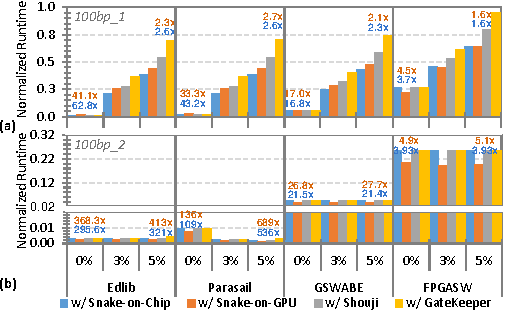
\includegraphics[width=1\linewidth]{figures/Figure5-Oct2020.pdf}}
\caption{\alser{Normalized end-to-end execution time of a pre-alignment filter (Snake-on-Chip, Snake-on-GPU, Shouji, and GateKeeper) combined with a sequence aligner (Edlib, Parasail, GSWABE, and FPGASW). {Each execution time value is normalized to that of the corresponding sequence aligner {without} pre-alignment filtering.}
We use two datasets, (a) \texttt{100bp\_1} and (b) \texttt{100bp\_2}, over a wide range of edit distance thresholds (0\%-10\% of the sequence length, 100 bp). We present two end-to-end speedup {values} for edit distance thresholds of 0\% and 5\%. The {top} speedup {value} {(in orange)} is the speedup gained from integrating Snake-on-GPU with the corresponding sequence aligner. The {bottom} speedup {value} {(in blue)} represents the speedup gained from integrating Snake-on-Chip with the corresponding sequence aligner.}}
\label{fig:Snake-on-Chip}
\end{figure}




%We now examine the execution time of SneakySnake, Parasail, and SneakySnake integrated with Parasail using long reads, as we show in Fig. 10. We run both SneakySnake and Parasail using two sets (Set\_5 and Set\_6) of long reads and 40 CPU threads. We run SneakySnake with $t$ = $y$ = (E+500), where $t$ is the width of the chip maze of each subproblem, $y$ is the number of iterations performed to solve each subproblem, and $E$ is the edit distance threshold. We choose the values of $t$ and $y$ to be less than the sequence length to prevent SneakySnake from examining the entire chip maze, which helps to achieve fast filtering at the cost of a slight increase in the number of falsely-accepted pairs (with a 0\% false reject rate). We also choose the values of $t$ and $y$ to be more than E to prevent the chip maze to have complete rows of obstacles based on Equation 1 in the main paper. 
%We experimentally evaluate the effect of varying the values of $t$ and $y$ on both the accuracy and execution time of short sequence filtering and alignment in \url{https://github.com/CMU-SAFARI/SneakySnake/tree/master/Evaluation\%20Results}. 
%We use a wide range of edit distance thresholds, up to 20\% of the sequence length. 

%Based on Fig. 10, we make two key observations. (1) Using Set\_5 and Set\_6, SneakySnake makes Parasail significantly faster (by 58.2-708.4$\times$ and by 50.9-978.8$\times$, respectively) than Parasail alone in detecting dissimilar pairs of long sequences, even at high edit distance thresholds (up to $E$=501 for Set\_5 and up to $E$=5010 for Set\_6, which result in building and examining 1003 and 10021 rows, respectively, for each chip maze of the SneakySnake algorithm). (2) As the number of similar sequence pairs increases (at E > 501 for Set\_5 and at E > 5010 for Set\_6), the benefits of integrating SneakySnake with Parasail in reducing the end-to-end execution time becomes less. As 89\% and 94\% of the input sequence pairs passed SneakySnake to Parasail using Set\_5 and Set\_6, respectively, integrating SneakySnake with Parasail shows almost the same end-to-end execution time of Parasail alone. This is expected, as each sequence pair that passed SneakySnake is examined unnecessarily twice (i.e., once by SneakySnake and once by Parasail). 
%We provide the exact values of all evaluation results in \url{https://github.com/CMU-SAFARI/SneakySnake/tree/master/Evaluation\%20Results}.

\subsection{{Effect} of SneakySnake on Long Sequence Alignment}
{We} examine the benefits of integrating SneakySnake with Parasail~\citep{daily2016parasail} and KSW2~\citep{suzuki2018introducing, li2018minimap2} {for long sequence alignment} (\texttt{100Kbp}). 
We run Parasail as nw\_banded. We run KSW2 as extz2\_sse, a global alignment implementation that is parallelized using the Intel SSE instructions{. KSW2} uses heuristics~\citep{suzuki2018introducing} to improve the alignment time. We run SneakySnake with Parasail using 40 CPU threads. We run SneakySnake with KSW2 using a single CPU thread (as KSW2 does not support multithreading). We use a wide range of edit distance thresholds, up to 20\% of the sequence length.

Based on Table \ref{table:1}, we make two key observations. (1) SneakySnake {accelerates} Parasail and KSW2 by 50.9-979$\times$ and 3.8-91.7$\times$, respectively, even at high edit distance thresholds (up to $E$=5010 (5\%), which results in building and examining a chip maze of 10,021 rows for each sequence pair).
(2) As the number of similar sequence pairs increases, the {performance benefit} of integrating SneakySnake with Parasail and KSW2 in reducing the end-to-end execution time {reduces}. 
{When Parasail and KSW2 examine 94\% and 73\% of the input sequence pairs (SneakySnake filters out the rest of the sequence pairs), respectively, SneakySnake provides slight or no performance benefit to the end-to-end execution time of the sequence aligner alone}. 
This is expected, as each sequence pair that passes SneakySnake is examined unnecessarily twice (i.e., once by SneakySnake and once by sequence aligner). We provide more details on this evaluation for both \texttt{10Kbp} and \texttt{100Kbp} in Supplementary Materials, Section 10.3.
We observe that SneakySnake accelerates Parasail and KSW2 by 276.9$\times$ and 31.7$\times$ on average, respectively, when {sequence alignment examines at most 73\% of the input sequence pairs}.

We conclude that {when SneakySnake filters out more than 27\% of the input sequence pairs, integrating SneakySnake with long sequence aligners is always beneficial and sometimes reduces the end-to-end execution time by one to two orders of magnitude (depending on the edit distance threshold and how fast the sequence aligner examines the input sequence pairs compared to SneakySnake) without the need for hardware accelerators}.


\begin{table}[H]
\caption{The end-to-end execution time (in seconds) of SneakySnake integrated with Parasail (40 CPU threads) and KSW2 (single threaded) using long reads (\texttt{100Kbp}).}
\label{table:1}
\centering
\begin{tabularx}{\linewidth}{c|rrrrr}
\hline
\textit{\textbf{E}} & \multicolumn{1}{l}{\textbf{Parasail}} & \multicolumn{1}{l}{\textbf{SS+Parasail}} & \multicolumn{1}{l}{\textbf{KSW2}} & \multicolumn{1}{l}{\textbf{SS+KSW2}} &  
\begin{minipage}[c] [.7cm] [c] {0.15\columnwidth}%
\centering
\textbf{SS Accept Rate} %
\end{minipage}
\\ \hline
0.01\% & 84.0 & \textbf{0.23} & 1380.2 & \textbf{15.1} & 0\% \\
0.3\% & 2,756.3 & \textbf{2.8} & 8,215.5 & \textbf{135.4} & 0\% \\
5.0\% & 37,492.3 & \textbf{736.5} & 100,178.3 & \textbf{26,261.4} & 0\% \\
10.7\% & 81,881.6 & \textbf{49,322.1} & 204,135.3 & \textbf{184,312.5} & 57\% \\
10.8\% & 82,646.1 & \textbf{63,756.0} & 206,041.4 & 225,815.2 & 73\% \\
11.0\% & 84,098.7 & \textbf{83,437.5} & 209,662.8 & 287,206.8 & 94\% \\
12.0\% & 91,744.1 & 95,533.6 & 228,723.1 & 325,966.0 & 100\% \\
20.0\% & 152,906.8 & 157,982.0 & 381,205.1 & 544,282.1 & 100\% \\ \hline
\end{tabularx}
\end{table}


%\begin{table}[H]
%\caption{The end-to-end execution time (in seconds) of SneakySnake integrated with Parasail (40 CPU threads) and KSW2 (single threaded) using long reads (\texttt{100Kbp}).}
%\label{table:1}
%\centering
%\begin{tabularx}{\linewidth}{c|rrrrr}
%ine
%\textit{\textbf{E}} & \multicolumn{1}{l}{\textbf{Parasail}} & \multicolumn{1}{l}{\textbf{SS+Parasail}} & \multicolumn{1}{l}{\textbf{KSW2}} & \multicolumn{1}{l}{\textbf{SS+KSW2}} &  
%\begin{minipage}[c] [.7cm] [c] {0.15\columnwidth}%
%\centering
%\textbf{SS Accept Rate} %
%\end{minipage}
%\\ ine
%0.01\% & 84.0 & \textbf{0.23} \small{(351.5$\times$)} & 1380.2 & \textbf{15.1} \small{(91.7$\times$)} & 0\% \\
%0.3\% & 2,756.3 & \textbf{2.8} \small{(979$\times$)} & 8,215.5 & \textbf{135.4} \small{(60.6$\times$)} & 0\% \\
%5.0\% & 37,492.3 & \textbf{736.5} \small{(50.9$\times$)} & 100,178.3 & \textbf{26,261.4} \small{(3.8$\times$)} & 0\% \\
%10.7\% & 81,881.6 & \textbf{49,322.1} \small{(1.7$\times$)} & 204,135.3 & \textbf{184,312.5} \small{(1.1$\times$)} & 57\% \\
%10.8\% & 82,646.1 & \textbf{63,756.0} \small{(1.3$\times$)} & 206,041.4 & 225,815.2 \small{(0.91$\times$)} & 73\% \\
%11.0\% & 84,098.7 & \textbf{83,437.5} \small{(1$\times$)} & 209,662.8 & 287,206.8 \small{(0.73$\times$)} & 94\% \\
%12.0\% & 91,744.1 & 95,533.6 \small{(0.96$\times$)} & 228,723.1 & 325,966.0 \small{(0.7$\times$)} & 100\% \\
%20.0\% & 152,906.8 & 157,982.0 \small{(0.97$\times$)} & 381,205.1 & 544,282.1 \small{(0.7$\times$)} & 100\% \\ ine
%\end{tabularx}
%\end{table}


\subsection{{Effect} of SneakySnake on Read Mapping}
\alser{After confirming the benefits of the different implementations of the SneakySnake algorithm, {we} evaluate the overall benefits of integrating SneakySnake with minimap2 (2.17-r974-dirty, 22 January 2020) \citep{li2018minimap2}. 
We select minimap2 for two main reasons. (1) It is a state-of-the-art read mapper that includes efficient methods (i.e., minimizers and seed chaining) for accelerating read mapping. (2) It utilizes a banded global sequence alignment algorithm (KSW2, implemented as \emph{extz2\_sse}) that is parallelized and accelerated using both the Intel SSE instructions and heuristics \citep{suzuki2018introducing} to improve the alignment time.
We map all reads from ERR240727\_1 (100 bp) to GRCh37 with edit distance thresholds of 0\% and 5\% of the sequence length. 
{We run minimap2 using --sr mode (short read mapping) and the default parameter values.}
We replace the seed chaining %(lines 305 to 358 of \emph{map.c} file) 
of minimap2 with SneakySnake.
In these experiments, we ensure that we maintain the \emph{same} reported mappings for both tools. 
We make two observations. 
(1) SneakySnake and the minimap2's aligner (KSW2) together are at least 6.83$\times$ (from 246 seconds to 36 seconds) and 2.51$\times$ (from 338 seconds to 134.67 seconds) faster than the minimap2's seed chaining and the minimap2's aligner together for edit distance thresholds of 0\% and 5\%, respectively. 
(2) The mapping time of minimap2 reduces by a factor of up to 2.01$\times$ (from 418 seconds to 208 seconds) and 1.66$\times$ (from 510 seconds to 306.67 seconds) after integrating SneakySnake with minimap2 for edit distance thresholds of 0\% and 5\%, respectively.}

{We conclude that SneakySnake is {very} beneficial even for minimap2, a state-of-the-art read mapper, which uses minimizers, seed chaining, and SIMD-accelerated banded alignment.
This promising result motivates us to explore in detail accelerating minimap2 using Snake-on-GPU and Snake-on-Chip in our future research.}
%After confirming the benefits of integrating SneakySnake and Snake-on-Chip with sequence aligners, we now evaluate the overall benefits of integrating SneakySnake and Snake-on-Chip with the mrFAST (version 2.6.1) read mapper \citep{alkan2009personalized}. We select mrFAST for two main reasons. (1) It already includes the Adjacency Filter \citep{xin2013accelerating} as a pre-alignment step, so it constitutes a state-of-the-art baseline. (2) It utilizes a banded Levenshtein edit distance algorithm \citep{ukkonen1985algorithms} that is parallelized using the Intel SSE instructions, and thus it utilizes the capabilities of state-of-the-art hardware. Fig. \ref{fig:mrFAST} presents the effect of SneakySnake and Snake-on-Chip on the overall mapping time, when all reads from ERR240727\_1 (100 bp) are mapped to GRCh37 with edit distance thresholds of 0\% to 5\%. We make two observations. (1) SneakySnake and Snake-on-Chip are at least 10.8$\times$ and 675.1$\times$ faster than mrFAST's banded Levenshtein edit distance algorithm. (2) The verification time of mrFAST reduces by a factor of up to 2.93$\times$ and 7.57$\times$ after replacing the Adjacency Filter with SneakySnake and Snake-on-Chip, respectively, as the pre-alignment filtering step.

%\begin{figure}
%\centerline{\includegraphics[width=0.8\linewidth]{figures/SneakySnake-mrFast.pdf}}
%\caption{Normalized end-to-end execution time of mrFAST (version 2.6.1) mapper combined with SneakySnake and Snake-on-Chip. We use mrFAST to map all reads from ERR240727\_1 (100 bp) to the human reference genome, GRCh37, over edit distance thresholds of 0\%-5\% of the sequence length, 100 bp. We present the end-to-end speedup rates that SneakySnake and Snake-on-Chip provide for mrFAST.}
%\label{fig:mrFAST}
%\end{figure}


\section{Discussion and Future Work} \label{sec:conclusion}
We {demonstrate {that} we can} convert {the} approximate string matching problem into an instance of the single net routing problem. 
We {show how to do so and} propose a new algorithm that solves the single net routing problem and acts as a new pre-alignment filtering algorithm, {called} SneakySnake. 
%We demonstrate that the concept of pre-alignment filtering provides substantial benefits {to} existing and future sequence alignment algorithms and read mappers {for both short and long sequences}. 
%Many of the existing acceleration efforts either simplify the scoring function, or only take into account accelerating the computation of the DP matrix without supporting the backtracking step. 
SneakySnake offers the ability to make the best use of existing aligners without sacrificing any of their capabilities (e.g., configurable scoring functions and backtracking), as it does not modify or replace the alignment step. %Our algorithm supports CPU multithreading {and it }does not exploit any SIMD-enabled CPU instructions or vendor-specific processor. This makes it attractive and cost-effective given a limited{-resource} environment. 
SneakySnake improves the accuracy of pre-alignment filtering by up to four orders of magnitude compared to {three} state-of-the-art pre-alignment filters, Shouji, GateKeeper, and SHD. The addition of SneakySnake as a pre-alignment filtering step {significantly} reduces the execution time of state-of-the-art CPU-based sequence aligners by up to an order {and two orders of magnitude using short and long sequences, respectively}. 
%{We} explore the use of hardware/software co-design and hardware {acceleration} to further accelerate our SneakySnake algorithm. 
{We introduce Snake-on-Chip and Snake-on-GPU, efficient and scalable FPGA and GPU based hardware accelerators of SneakySnake, respectively}. Snake-on-Chip and Snake-on-GPU achieve up to {one order and} two orders of magnitude speedup {over} state-of-the-art {CPU- and hardware-based sequence aligners, respectively}.

One direction to further improve the performance of Snake-on-Chip is to discover the possibility of performing the SneakySnake calculations {near where huge amounts} of genomic data resides. Conventional computing requires the movement of genomic sequence pairs from the memory to the CPU processing cores (or to the {GPU or FPGA chips}), using slow and energy-hungry buses, such that cores can apply sequence alignment algorithm on the sequence pairs. 
Performing SneakySnake inside modern memory devices {via processing in memory}~\citep{mutlu2019processing, ghose2019processing} can alleviate this high communication cost by enabling simple arithmetic/logic operations very close to where the data resides, with high bandwidth, low latency{, and low energy}. However, this requires re-designing the hardware architecture of Snake-on-Chip to leverage the supported operations in such modern memory devices. 
%This also encourages us to explore the possibility of accelerating sequence alignment algorithms for longer sequences (few tens of thousands of characters) which is mainly limited by 1) the data transfer rate of the communication link (i.e., PCIe) and 2) large edit distance thresholds.


% \section*{Acknowledgements}
% Text Text  Text Text
\vspace{-6 pt}
\section*{Funding}
This work is supported by gifts from Intel [to O.M.]; VMware [to O.M.]; {a Semiconductor Research Corporation grant [to O.M.];} and an EMBO Installation Grant [IG-2521 to C.A.].\\
\vspace{-20 pt}

\bibliographystyle{natbib}
% \bibliographystyle{achemnat}
% \bibliographystyle{plainnat}
% \bibliographystyle{abbrv}
% \bibliographystyle{bioinformatics}
% \bibliographystyle{plain}

\bibliography{document}

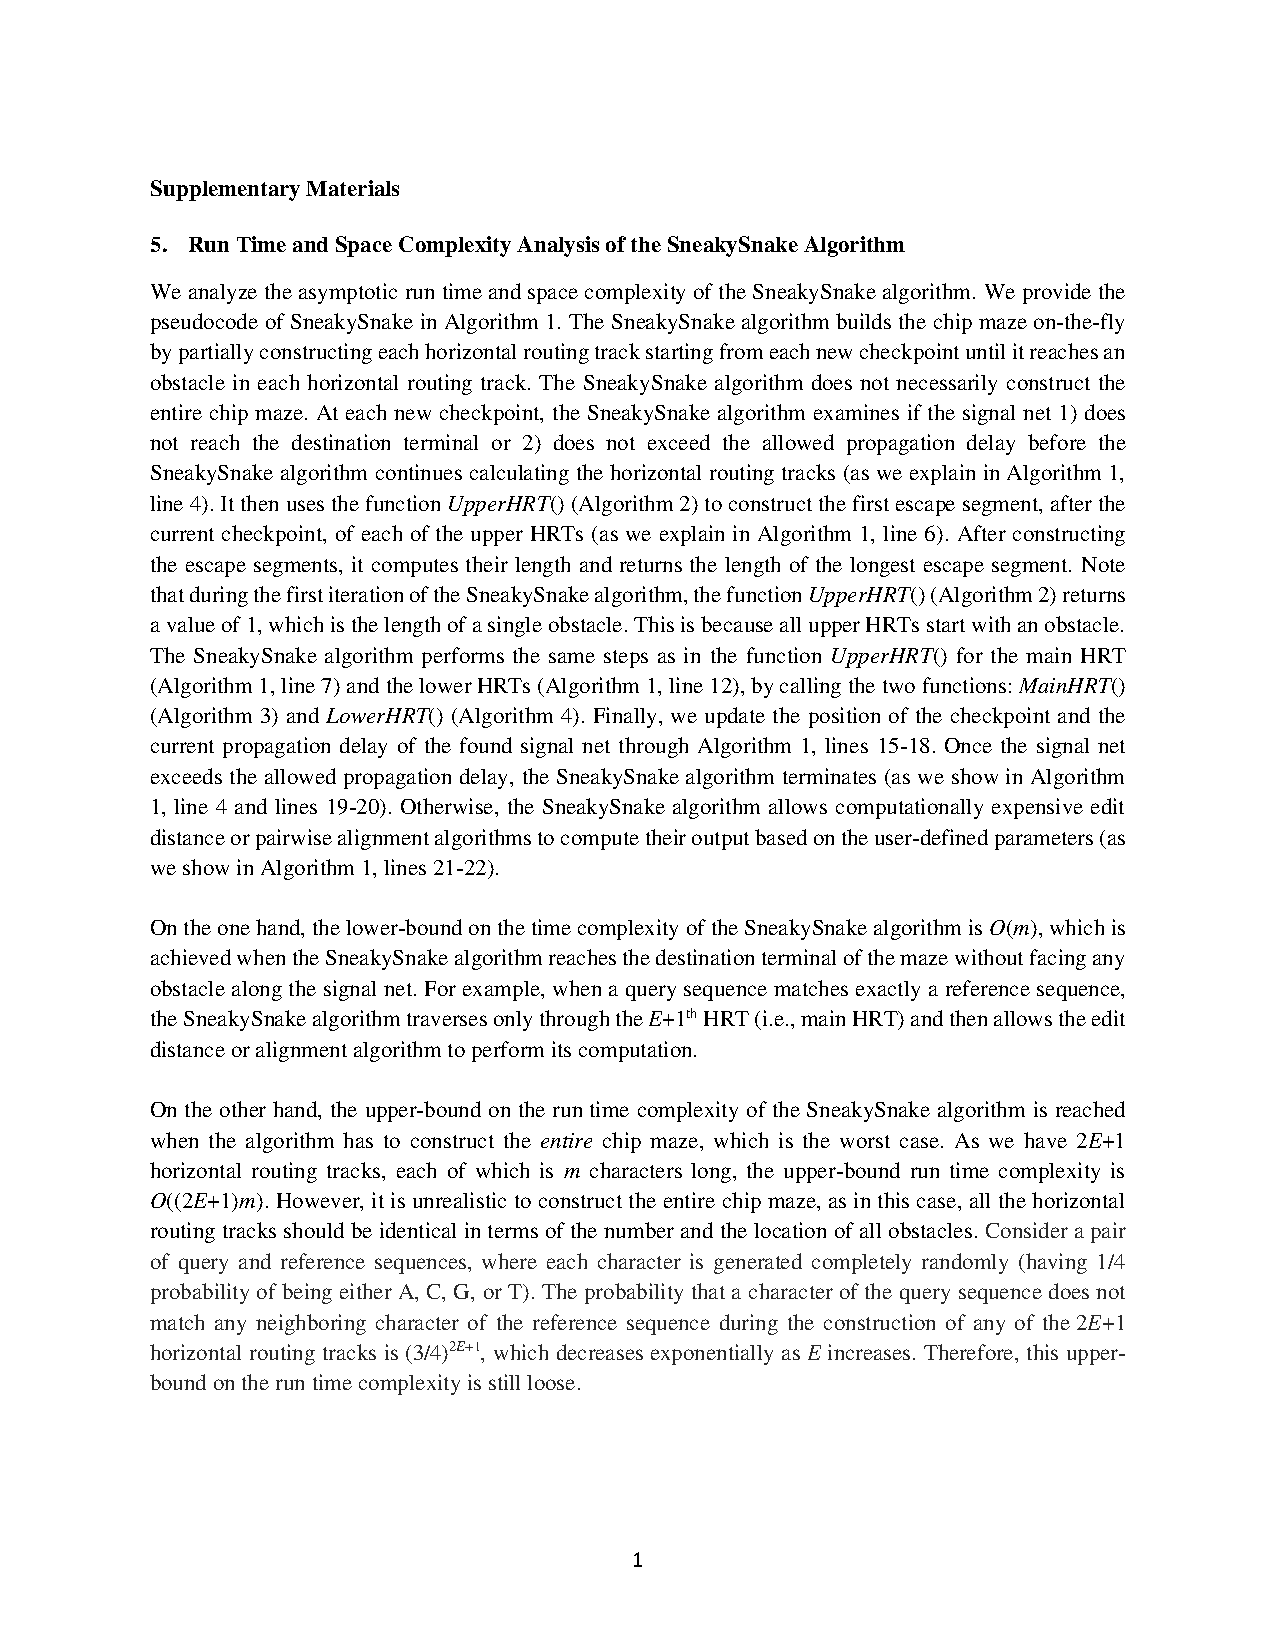
\includepdf[pages=-]{SneakySnakeSuppMaterials23Nov2020}


\end{document}
